% ============================================================
% SecureAuth -- Rapport de développement
% Compilation : voir docs/rapport/README.md (latexmk -pdf)
% ============================================================
\documentclass[12pt,a4paper]{report}

\usepackage[utf8]{inputenc}
\usepackage[T1]{fontenc}
\usepackage{lmodern}
\usepackage[french]{babel}
\usepackage[a4paper,margin=2.5cm,headheight=15pt]{geometry}
\usepackage{xcolor}
\usepackage{graphicx}
\usepackage{adjustbox}
\usepackage{amsmath,amssymb}
\usepackage{booktabs,array,longtable}
\usepackage{float}
\usepackage{caption}
\usepackage{fancyhdr}
\usepackage{titlesec}
\usepackage{tikz}
\usetikzlibrary{arrows.meta,calc,positioning,shapes.multipart,shapes.geometric,backgrounds}
\usepackage[colorlinks=true,linkcolor=titreblue,urlcolor=titreblue,citecolor=titreblue,
            pdftitle={SecureAuth -- Rapport de conception},
            pdfauthor={Khalil Hnich, Houssem Ben Khamou}]{hyperref}

\definecolor{titreblue}{rgb}{0,0,0.65}

% caractères Unicode utilisés dans les figures
\DeclareUnicodeCharacter{2192}{\ensuremath{\rightarrow}}
\DeclareUnicodeCharacter{2248}{\ensuremath{\approx}}
\DeclareUnicodeCharacter{2265}{\ensuremath{\geq}}

% ============================================================
% Petites macros TikZ pour dessiner les diagrammes UML du rapport
% (acteurs, classes, séquence) sans aucun outil externe.
% ============================================================

\definecolor{umlgrey}{gray}{0.55}
\definecolor{umlfill}{gray}{0.93}

\tikzset{
  >=Stealth,
  uml/.style={font=\footnotesize\sffamily},
  % ---------- cas d'utilisation ----------
  uc/.style={ellipse, draw=black, fill=white, align=center, font=\scriptsize\sffamily,
             minimum height=0.95cm, text width=2.9cm, inner sep=1pt},
  ucint/.style={uc, fill=umlfill},
  assoc/.style={draw=black},
  incl/.style={draw=black, dashed, -{Stealth[length=2mm]}},
  gener/.style={draw=black, -{Triangle[open, length=3mm, width=3mm]}},
  rellabel/.style={font=\fontsize{6}{7}\selectfont\sffamily, fill=white, inner sep=1pt, sloped},
  % ---------- classes ----------
  cls/.style={rectangle split, rectangle split parts=3, draw=black, fill=white,
              rectangle split part align={center,left,left}, font=\scriptsize\sffamily,
              inner xsep=5pt, inner ysep=3pt, text width=3.7cm},
  clsenum/.style={cls, rectangle split parts=2, rectangle split part align={center,left}, fill=umlfill},
  mult/.style={font=\fontsize{6}{7}\selectfont\sffamily, inner sep=1.5pt},
  % ---------- séquences ----------
  lifebox/.style={draw=black, fill=white, align=center,
                  font=\scriptsize\sffamily, inner sep=3pt, minimum height=0.7cm, text width=2.5cm},
  lifeline/.style={draw=black!60, dashed, thin},
  msg/.style={-{Stealth[length=2mm]}, draw=black},
  retmsg/.style={-{Stealth[length=2mm, open]}, dashed, draw=black},
  msgl/.style={above, font=\scriptsize\sffamily, align=center, inner sep=1pt, fill=white, fill opacity=0.85, text opacity=1},
  fragbox/.style={draw=black!60},
  fragtab/.style={draw=black!60, fill=white, font=\scriptsize\sffamily, inner sep=2pt, anchor=north west},
  fragcond/.style={font=\scriptsize\sffamily, anchor=west},
}

% ---------- acteur (bonhomme) : \actor{nom}{x,y}{libellé} ----------
\newcommand{\actor}[3]{%
  \begin{scope}[shift={(#2)}]
    \draw (0,0.62) circle (0.17);
    \draw (0,0.45)--(0,-0.05);
    \draw (-0.3,0.3)--(0.3,0.3);
    \draw (0,-0.05)--(-0.22,-0.5);
    \draw (0,-0.05)--(0.22,-0.5);
  \end{scope}
  \node[inner sep=0, minimum width=0.7cm, minimum height=1.1cm] (#1) at ($(#2)+(0,0.05)$) {};
  \node[font=\scriptsize\sffamily\bfseries, align=center, below=0.5cm of #1, text width=2.4cm] {#3};
}

% ---------- séquences ----------
% Les lignes de vie sont désignées par un identifiant ; \lx{id} donne leur abscisse (en cm).
\newcommand{\lx}[1]{\csname lx@#1\endcsname}
\newcommand{\seqbegin}{\def\cury{-0.35}\gdef\lifelist{}\def\seqk{0.85}}
\newcommand{\life}[3]{%
  \expandafter\gdef\csname lx@#1\endcsname{#2}%
  \node[lifebox] at (#2,0) {#3};
  \ifx\lifelist\empty\xdef\lifelist{#2}\else\xdef\lifelist{\lifelist,#2}\fi
}
\newcommand{\seqend}{%
  \pgfmathsetmacro{\yend}{\cury-0.5}%
  \begin{scope}[on background layer]
    \foreach \lfx in \lifelist {\draw[lifeline] (\lfx,-0.35)--(\lfx,\yend);}
  \end{scope}
}
% message : \msg[pas]{de}{vers}{libellé}   (\ret : retour en pointillé)
\newcommand{\msg}[4][0.8]{%
  \pgfmathsetmacro{\cury}{\cury-#1*\seqk}%
  \pgfmathsetmacro{\mxa}{\lx{#2}}\pgfmathsetmacro{\mxb}{\lx{#3}}%
  \draw[msg] (\mxa,\cury)--(\mxb,\cury) node[msgl, pos=0.5] {#4};%
}
\newcommand{\ret}[4][0.8]{%
  \pgfmathsetmacro{\cury}{\cury-#1*\seqk}%
  \pgfmathsetmacro{\mxa}{\lx{#2}}\pgfmathsetmacro{\mxb}{\lx{#3}}%
  \draw[retmsg] (\mxa,\cury)--(\mxb,\cury) node[msgl, pos=0.5] {#4};%
}
% message sur soi-même : \selfmsg[pas]{ligne}{libellé}
\newcommand{\selfmsg}[3][0.8]{%
  \pgfmathsetmacro{\cury}{\cury-#1*\seqk}%
  \pgfmathsetmacro{\sx}{\lx{#2}}%
  \pgfmathsetmacro{\ya}{\cury-0.38}%
  \pgfmathsetmacro{\xb}{\sx+0.55}%
  \pgfmathsetmacro{\xc}{\sx+0.6}%
  \pgfmathsetmacro{\ym}{\cury-0.19}%
  \draw[msg] (\sx,\cury)--(\xb,\cury)--(\xb,\ya)--(\sx,\ya);%
  \node[font=\scriptsize\sffamily, anchor=west, align=left, inner sep=1.5pt, fill=white, fill opacity=0.85, text opacity=1] at (\xc,\ym) {#3};%
  \pgfmathsetmacro{\cury}{\cury-0.38}%
}
% fragment combiné : \fragbegin[marge]{id}{type}{ligne gauche}{ligne droite}{condition}
%                    \fragelse{id}{condition}   \fragend{id}
\newcommand{\fragbegin}[6][0.7]{%
  \pgfmathsetmacro{\cury}{\cury-0.3}%
  \pgfmathsetmacro{\fxl}{\lx{#4}-#1}\pgfmathsetmacro{\fxr}{\lx{#5}+#1}%
  \expandafter\xdef\csname fy@#2\endcsname{\cury}%
  \expandafter\xdef\csname fx1@#2\endcsname{\fxl}%
  \expandafter\xdef\csname fx2@#2\endcsname{\fxr}%
  \node[fragtab] (tab#2) at (\fxl,\cury) {#3};%
  \node[fragcond] at ($(tab#2.east)+(0.1,0)$) {#6};%
  \pgfmathsetmacro{\cury}{\cury-0.3}%
}
\newcommand{\fragelse}[2]{%
  \pgfmathsetmacro{\cury}{\cury-0.4}%
  \expandafter\let\expandafter\fxa\csname fx1@#1\endcsname
  \expandafter\let\expandafter\fxb\csname fx2@#1\endcsname
  \draw[fragbox, dashed] (\fxa,\cury)--(\fxb,\cury);%
  \pgfmathsetmacro{\xe}{\fxa+0.1}%
  \pgfmathsetmacro{\ye}{\cury-0.2}%
  \node[fragcond] at (\xe,\ye) {#2};%
  \pgfmathsetmacro{\cury}{\cury-0.25}%
}
\newcommand{\fragend}[1]{%
  \pgfmathsetmacro{\yfe}{\cury-0.3}%
  \expandafter\let\expandafter\fxa\csname fx1@#1\endcsname
  \expandafter\let\expandafter\fxb\csname fx2@#1\endcsname
  \expandafter\let\expandafter\fya\csname fy@#1\endcsname
  \draw[fragbox] (\fxa,\fya) rectangle (\fxb,\yfe);%
  \pgfmathsetmacro{\cury}{\cury-0.15}%
}

% ---------- classes : \umlclass[options]{nom}{style}{titre}{attributs}{méthodes} ----------
\newcommand{\umlclass}[6][]{%
  \node[#3, #1] (#2) {#4\nodepart{second}#5\nodepart{third}#6};%
}
\newcommand{\umlenum}[4][]{%
  \node[clsenum, #1] (#2) {#3\nodepart{second}#4};%
}

% Figure UML mise à l'échelle de la largeur de ligne
\newcommand{\umlfig}[2][0.62]{%
  \begingroup\hyphenpenalty=10000 \exhyphenpenalty=10000
  \noindent\adjustbox{max width=\linewidth, max totalheight=#1\textheight, center}{\input{#2}}%
  \endgroup}


\newcommand{\code}[1]{\texttt{\NoAutoSpacing #1}}

% --- titres : même allure que le rapport de référence ---
\titleformat{\chapter}[display]{\normalfont\huge\color{titreblue}}{\Huge Chapitre~\thechapter}{22pt}{\Huge}
\titlespacing*{\chapter}{0pt}{40pt}{30pt}
\titleformat{\section}{\normalfont\Large\bfseries\color{titreblue}}{\thesection}{0.6em}{}
\titleformat{\subsection}{\normalfont\large\bfseries\color{titreblue}}{\thesubsection}{0.6em}{}

% --- en-têtes et pieds de page ---
\pagestyle{fancy}
\fancyhf{}
\renewcommand{\chaptermark}[1]{\markboth{\MakeUppercase{Chapitre \thechapter.\ #1}}{}}
\fancyhead[L]{\small\leftmark}
\fancyhead[R]{\small\thepage}
\fancyfoot[C]{\small SecureAuth -- TEK-UP}
\renewcommand{\headrulewidth}{0.4pt}
\renewcommand{\footrulewidth}{0.4pt}
\fancypagestyle{plain}{\fancyhf{}\fancyfoot[C]{\small\thepage}\renewcommand{\headrulewidth}{0pt}\renewcommand{\footrulewidth}{0pt}}

\captionsetup{labelsep=endash}
\setlength{\emergencystretch}{2em}

\begin{document}

% ================= PAGE DE GARDE =================
\begin{titlepage}
  \centering
  \vspace*{0.5cm}
  
\includegraphics[width=4.6cm]{img/tek_up_logo.jpg}\\[0.4cm]
  {\large Université TEK-UP}\\[0.15cm]
  {\normalsize Module Cybersécurité -- Projet 2}\\[2.2cm]

  {\Huge RAPPORT DE CONCEPTION\\[0.3cm] \LARGE et de développement}\\[1.4cm]
  {\Large\bfseries SecureAuth}\\[0.3cm]
  {\large\itshape Coffre-fort de documents classifiés :\\
   système sécurisé d'authentification et de cryptographie}\\[2.4cm]

  {\Large\bfseries Équipe de développement}\\[0.4cm]
  Khalil Hnich\\
  Houssem Ben Khamou\\[0.8cm]
  {\large\bfseries Encadrant}\\[0.2cm]
  Oussema Bakali
  \vfill
  {\bfseries Année universitaire 2026--2027}\\[0.2cm]
  Octobre 2026
\end{titlepage}

\pagenumbering{roman}
\setcounter{page}{1}
\tableofcontents
\clearpage
\listoffigures
\clearpage
\listoftables
\clearpage
\pagenumbering{arabic}

% =====================================================
\chapter{Introduction et Contexte du Projet}
% =====================================================

\section{Introduction}

SecureAuth est une application Web qui protège les documents classifiés d'une agence fictive. Elle décide côté serveur qui a le droit de lire quel document, elle chiffre chaque document avant de le ranger en base, et elle note chaque passage devant un contrôle d'accès dans un journal que l'on ne peut pas modifier sans que cela se voie.

Le projet est le sujet n\textdegree{}2 du module Cybersécurité de TEK-UP, intitulé \og Système sécurisé d'authentification et de cryptographie \fg. Il se déroule sur six semaines. L'idée de départ est simple : se connecter avec un mot de passe ne suffit pas à protéger des informations sensibles. Le vrai travail est de décider ce que chaque utilisateur peut lire une fois connecté, de le faire respecter par le serveur, et de pouvoir le prouver.

Chaque document porte un niveau de classification (PUBLIC, CONFIDENTIEL, SECRET ou TRÈS SECRET) et chaque agent porte une habilitation sur la même échelle. Lire un document demande deux choses : une habilitation au moins égale à sa classification, et la présence de l'agent sur la liste d'accès du document. L'administrateur gère les comptes mais ne lit aucun document.

\section{Problématique}

Un système qui manipule des documents sensibles est exposé à plusieurs menaces. Un mot de passe peut être deviné ou volé, un cookie de session peut être rejoué, un utilisateur peut essayer de lire un document qui ne lui est pas destiné en modifiant simplement l'adresse dans son navigateur. Un administrateur trop puissant est lui aussi un risque : s'il peut tout lire, la compromission de son compte compromet tout. Enfin, quelqu'un qui accède directement à la base de données peut lire les documents ou effacer les traces de ses actions.

La question à laquelle le projet répond est donc la suivante : comment construire une application où l'authentification, l'autorisation et la cryptographie se complètent, de façon qu'aucune de ces protections ne repose sur une seule barrière ?

\section{Besoins fonctionnels}

Le système doit permettre :
\begin{itemize}
  \item à un visiteur de s'inscrire avec un nom d'utilisateur, une adresse e-mail et un mot de passe, puis de se connecter, de se déconnecter et de changer son mot de passe ;
  \item de créer le premier administrateur uniquement en ligne de commande, jamais depuis l'interface ;
  \item de verrouiller un compte pendant quinze minutes après cinq échecs de connexion consécutifs ;
  \item à un agent de créer, de lister et de lire des documents texte classifiés, dans la limite de son habilitation ;
  \item à un agent de partager un document qu'il a créé en ajoutant ou en retirant des agents de sa liste d'accès ;
  \item à l'administrateur de lister les comptes, de modifier une habilitation, d'activer ou de désactiver un compte, et de consulter la liste d'accès d'un document sans jamais voir son contenu ;
  \item à l'administrateur de consulter le journal d'audit et d'en vérifier l'intégrité ;
  \item d'enregistrer dans le journal les événements de sécurité (inscription, connexion, échec, lecture, refus d'accès, changement d'habilitation, etc.) sans y écrire de mot de passe, de contenu de document ni de clé.
\end{itemize}

\section{Besoins non fonctionnels}

\begin{itemize}
  \item Une vérification de mot de passe prend à peu près le même temps que le compte existe ou non, pour ne pas révéler les comptes valides.
  \item Un document non autorisé donne une réponse 404, jamais 403 : le système ne confirme pas l'existence d'un document classifié.
  \item Le journal reste cohérent même avec plusieurs processus qui écrivent en parallèle.
  \item L'application ne tourne pas en \emph{root} et la base n'est jamais accessible depuis l'extérieur.
  \item Les secrets (clés AES et HMAC, mots de passe de la base) ne sont jamais dans le dépôt Git ; l'application refuse de démarrer si une clé manque ou est mal formée.
  \item Le déploiement se fait avec Docker Compose, sous Windows comme sous Linux.
  \item Les tests automatiques s'exécutent sans conteneur, avec une base en mémoire et un faux Redis.
  \item Le code est modulaire : toutes les décisions d'accès aux documents passent par un seul module.
\end{itemize}

% =====================================================
\chapter{Organisation du Projet}
% =====================================================

\section{Démarche}

Le sujet impose six phases, une par semaine. L'équipe les a suivies dans l'ordre. Une fonctionnalité de sécurité est considérée comme terminée lorsqu'elle a un test automatique qui passe, une vérification manuelle décrite avec son résultat attendu, et une preuve utilisable dans le rapport (capture, extrait du journal ou sortie de commande). Cette règle vient du module : un résultat de sécurité doit être démontré, pas seulement affirmé. Le dépôt contient aujourd'hui plus de trois cents tests automatiques et un script qui rejoue les attaques contre l'application réellement déployée.

Les décisions ont été prises avant de coder et consignées dans un cahier des charges (version 1.0, octobre 2026) : exigences fonctionnelles, exigences de sécurité, modèle de menace avec quatorze menaces et plan de vingt-cinq tests.

\begin{table}[H]
\centering
\begin{tabular}{@{}c l p{7.2cm}@{}}
\toprule
\textbf{Semaine} & \textbf{Phase} & \textbf{État actuel} \\
\midrule
1 & Conception et infrastructure & Terminée : Docker Compose, Nginx avec TLS, mini-PKI, MariaDB, Redis. \\
2 & Authentification & Terminée : inscription, connexion, déconnexion, mot de passe, sessions Redis, verrouillage après cinq échecs, journal d'audit. \\
3 & Autorisation et chiffrement & Terminée : règles d'accès, AES-256-GCM, espaces documents et administration, jeu de démonstration, ajout d'utilisateurs par l'administrateur, dépôt de fichiers PDF, DOC et DOCX. \\
4 & Tests de sécurité & Réalisés : les vingt-cinq cas, plus cinq cas pour les comptes créés par l'administrateur et les fichiers, par tests automatiques et par un script contre les vrais services. \\
5 & Corrections et durcissement & Terminée : limitation de débit, HSTS, conteneur applicatif en lecture seule, certificat corrigé. \\
6 & Livraison & Terminée : README, tests de sécurité, scénario de démonstration, rapport. \\
\bottomrule
\end{tabular}
\caption{Planning du projet et état d'avancement}
\end{table}

\section{Organisation de l'équipe}

L'équipe est composée de deux étudiants, Khalil Hnich et Houssem Ben Khamou, encadrés par Oussema Bakali. Tout le code est versionné dans un dépôt Git. Les deux membres participent à la conception, au développement et aux tests ; les choix techniques importants sont écrits dans le cahier des charges plutôt que laissés à la mémoire de chacun.

% =====================================================
\chapter{Architecture et Conception du Système}
% =====================================================

\section{Architecture globale}

L'application tourne dans quatre conteneurs Docker. Le navigateur ne parle qu'à Nginx, qui est le seul service dont les ports (80 et 443) sont publiés sur la machine. Nginx termine le chiffrement TLS puis transmet la requête à l'application Flask, servie par Gunicorn. Seule l'application peut joindre MariaDB et Redis, qui se trouvent sur un second réseau Docker déclaré \og interne \fg{} : ils n'ont aucun accès à Internet.

\begin{figure}[H]
\centering
\umlfig[0.35]{figures/deploy}
\caption{Architecture de déploiement : quatre conteneurs et deux réseaux}
\end{figure}

Les secrets sont injectés uniquement là où ils servent. L'application ne reçoit jamais le mot de passe \emph{root} de la base, et les clés de chiffrement viennent d'un fichier \code{.env} exclu de Git.

\section{Diagramme de Classes}

Le diagramme de classes montre les cinq tables de la base et leurs relations. Seule la référence d'un document reste en clair : son titre et son contenu sont chiffrés ensemble.

\begin{figure}[H]
\centering
\umlfig[0.58]{figures/class-domain}
\caption{Diagramme de classes -- SecureAuth}
\end{figure}

\textbf{Classes principales :}
\begin{itemize}
  \item \textbf{User} : un compte. Il garde l'empreinte Argon2id du mot de passe (jamais le mot de passe), son rôle (\code{user} ou \code{admin}), son habilitation de 0 à 3, son état actif ou désactivé, et les champs nécessaires au verrouillage (\code{failed\_attempts}, \code{locked\_until}).
  \item \textbf{SecureDocument} : un document classifié. Il a un identifiant public aléatoire (UUID) utilisé dans les adresses, une référence lisible, une classification, un propriétaire, et le texte chiffré avec son nonce de 12 octets.
  \item \textbf{DocumentAccess} : une ligne par agent autorisé à lire un document (le besoin d'en connaître). Elle garde aussi qui a accordé l'accès et quand.
  \item \textbf{AuditLog} : une ligne du journal. Chaque ligne contient l'empreinte de la précédente et sa propre empreinte HMAC-SHA256.
  \item \textbf{AuditChainHead} : une seule ligne qui mémorise la dernière entrée du journal. Elle permet de détecter la suppression des dernières lignes.
\end{itemize}

Un compte n'est jamais supprimé, seulement désactivé : supprimer l'auteur d'une ligne déjà signée casserait la signature du journal. De même, la date du journal est stockée avec les microsecondes, sinon la date relue en base serait différente de la date signée.

\section{Diagramme de Cas d'Utilisation}

Le diagramme de cas d'utilisation présente ce que chaque acteur peut faire. Les ellipses grises sont des cas internes, réutilisés par plusieurs fonctionnalités.

\begin{figure}[H]
\centering
\umlfig[0.8]{figures/uc-global}
\caption{Diagramme de cas d'utilisation -- SecureAuth}
\end{figure}

\textbf{Cas d'utilisation principaux :}
\begin{itemize}
  \item S'inscrire, se connecter, se déconnecter et changer son mot de passe ;
  \item lister, créer et lire des documents selon son habilitation ;
  \item partager un document que l'on a créé ;
  \item gérer les comptes et les habilitations (administrateur) ;
  \item consulter le journal d'audit et en vérifier l'intégrité (administrateur).
\end{itemize}

Trois points méritent d'être précisés. Lire un document passe toujours par le cas interne \og Vérifier les droits d'accès \fg{} : c'est le point de décision unique du projet. L'administrateur n'est associé à aucun cas de lecture de document, ce qui traduit la séparation des rôles. Enfin, le verrouillage du compte est une extension de la connexion : il ne se déclenche qu'après cinq échecs consécutifs.

\section{Diagramme de Séquence : Inscription}

Le diagramme de séquence suivant détaille ce qui se passe quand un visiteur envoie le formulaire d'inscription.

\begin{figure}[H]
\centering
\umlfig[0.62]{figures/seq-register}
\caption{Diagramme de séquence -- Inscription}
\end{figure}

\textbf{Description du fonctionnement :}

Le navigateur envoie le formulaire avec son jeton CSRF. La route Flask vérifie d'abord le jeton et la forme des champs ; si quelque chose ne va pas, le formulaire est renvoyé avec les erreurs. Sinon, elle passe les données au service d'authentification, qui commence par vérifier la politique de mot de passe : entre 12 et 128 caractères, différent du nom d'utilisateur, absent d'une liste de mots de passe courants.

Le service calcule ensuite l'empreinte Argon2id, \emph{avant} de regarder si le nom ou l'adresse e-mail existent déjà. C'est volontaire : l'opération dure environ 50 ms dans tous les cas, donc le temps de réponse ne révèle pas si un compte existe. Si le nom ou l'adresse sont déjà pris, l'utilisateur reçoit un message unique et volontairement vague (\og Inscription impossible avec ces informations \fg).

Si tout est correct, le compte est créé avec le rôle \code{user} et l'habilitation 0, et une ligne \code{REGISTER} est ajoutée au journal d'audit, signée par HMAC. L'utilisateur est redirigé vers la page de connexion. Un nouvel inscrit ne peut donc jamais devenir administrateur par ce formulaire.

\section{Technologies Utilisées}

La pile technique a été fixée au début du projet et n'a pas changé.

\begin{figure}[H]
\centering
\newcommand{\techlogo}[2]{\begin{tabular}[t]{@{}c@{}}\includegraphics[height=1.15cm]{img/logos/#1.pdf}\\[2pt]{\small #2}\end{tabular}}
\begin{tabular}{@{}ccccc@{}}
\techlogo{python}{Python 3.12} & \techlogo{flask}{Flask 3.1} & \techlogo{jinja}{Jinja2} & \techlogo{sqlalchemy}{SQLAlchemy} & \techlogo{gunicorn}{Gunicorn}\\[14pt]
\techlogo{nginx}{Nginx} & \techlogo{mariadb}{MariaDB 11.4} & \techlogo{redis}{Redis 7} & \techlogo{docker}{Docker Compose} & \techlogo{openssl}{OpenSSL}\\[14pt]
\techlogo{burp}{Burp Suite} & \techlogo{git}{Git} & \techlogo{latex}{\LaTeX} & &\\
\end{tabular}
\caption{Technologies utilisées dans le projet}
\end{figure}

\begin{itemize}
  \item \textbf{Application} : Python et Flask, avec Jinja2 pour les pages et SQLAlchemy pour accéder à la base. Aucune requête SQL n'est construite à la main, ce qui écarte l'injection SQL. Les formulaires utilisent Flask-WTF (jeton CSRF), les sessions Flask-Session et la limitation de débit Flask-Limiter.
  \item \textbf{Serveurs} : Gunicorn (trois processus, utilisateur non-root) exécute Flask. Nginx est le point d'entrée : TLS 1.2 et 1.3, redirection de HTTP vers HTTPS, en-têtes de sécurité.
  \item \textbf{Données} : MariaDB stocke les comptes, les documents chiffrés et le journal. Redis stocke les sessions côté serveur : le cookie ne contient qu'un identifiant aléatoire, et la déconnexion détruit réellement la session.
  \item \textbf{Cryptographie} : \code{argon2-cffi} pour les mots de passe (Argon2id), \code{cryptography} pour AES-256-GCM, le module standard \code{hmac} pour le journal. Aucun algorithme maison. OpenSSL sert à créer la mini-autorité de certification et le certificat du serveur.
  \item \textbf{Déploiement} : Docker Compose, avec deux réseaux dont un interne.
  \item \textbf{Tests} : \code{pytest} pour les tests automatiques ; Burp Suite, OpenSSL, curl et les outils de développement du navigateur pour les tests de sécurité de la semaine 4.
  \item \textbf{Documentation} : Git pour le dépôt, \LaTeX{} pour ce rapport et ses diagrammes.
\end{itemize}

Les icônes des logos proviennent du projet Simple Icons ; les marques appartiennent à leurs propriétaires respectifs.

% =====================================================
\chapter{Captures d'Écran de l'Application}
% =====================================================

Les captures de ce chapitre montrent les pages déjà réalisées. Elles ont été prises sur une instance locale avec un compte de démonstration (\code{alice}, habilitation SECRET) créé pour l'occasion.

\section{Page d'Inscription}

\begin{figure}[H]
\centering
\fbox{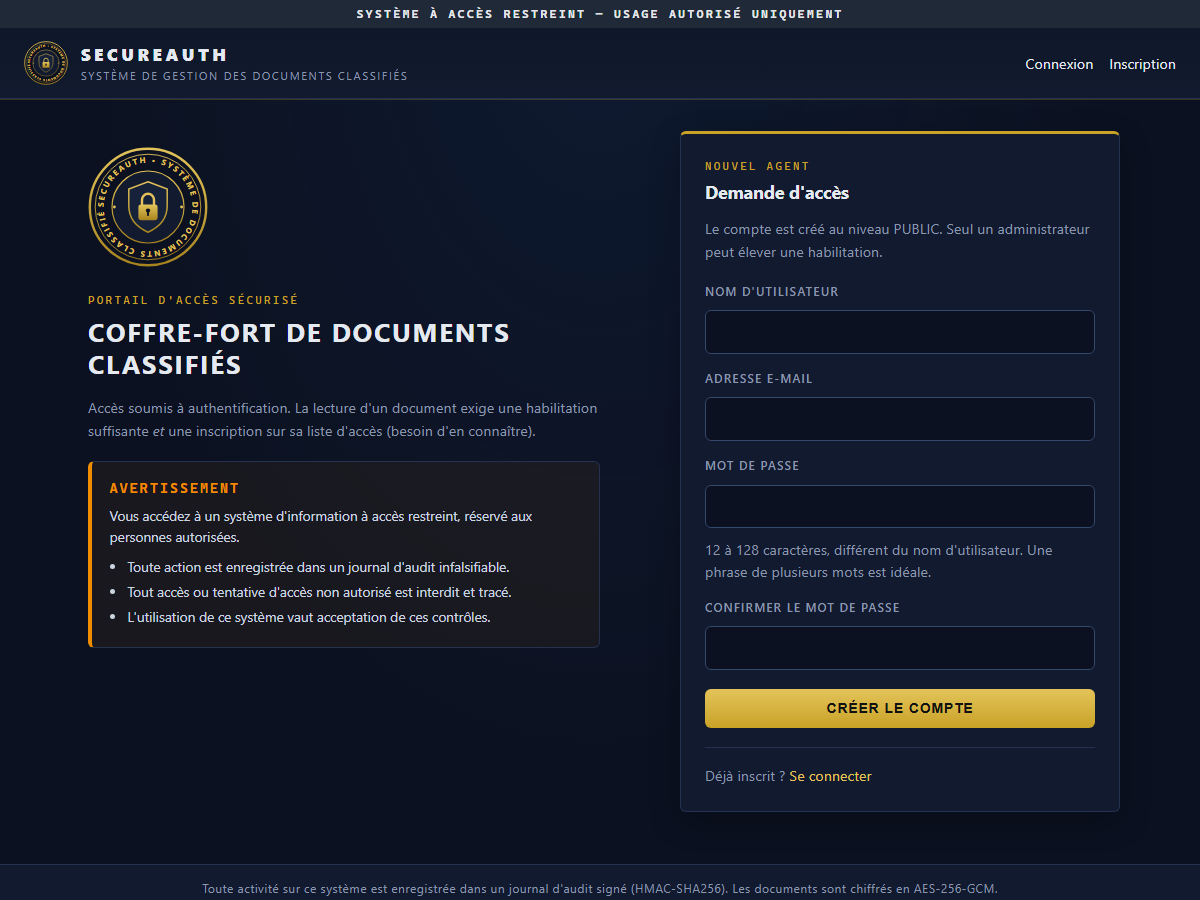
\includegraphics[width=0.88\linewidth]{img/captures/register.png}}
\caption{Formulaire d'inscription}
\end{figure}

Le formulaire demande le nom d'utilisateur, l'adresse e-mail, le mot de passe et sa confirmation. La page rappelle la règle de longueur (12 à 128 caractères) et précise que le compte est créé au niveau PUBLIC : seul un administrateur peut élever une habilitation. Un avertissement rappelle que toute action est enregistrée dans le journal d'audit.

\section{Page de Connexion}

\begin{figure}[H]
\centering
\fbox{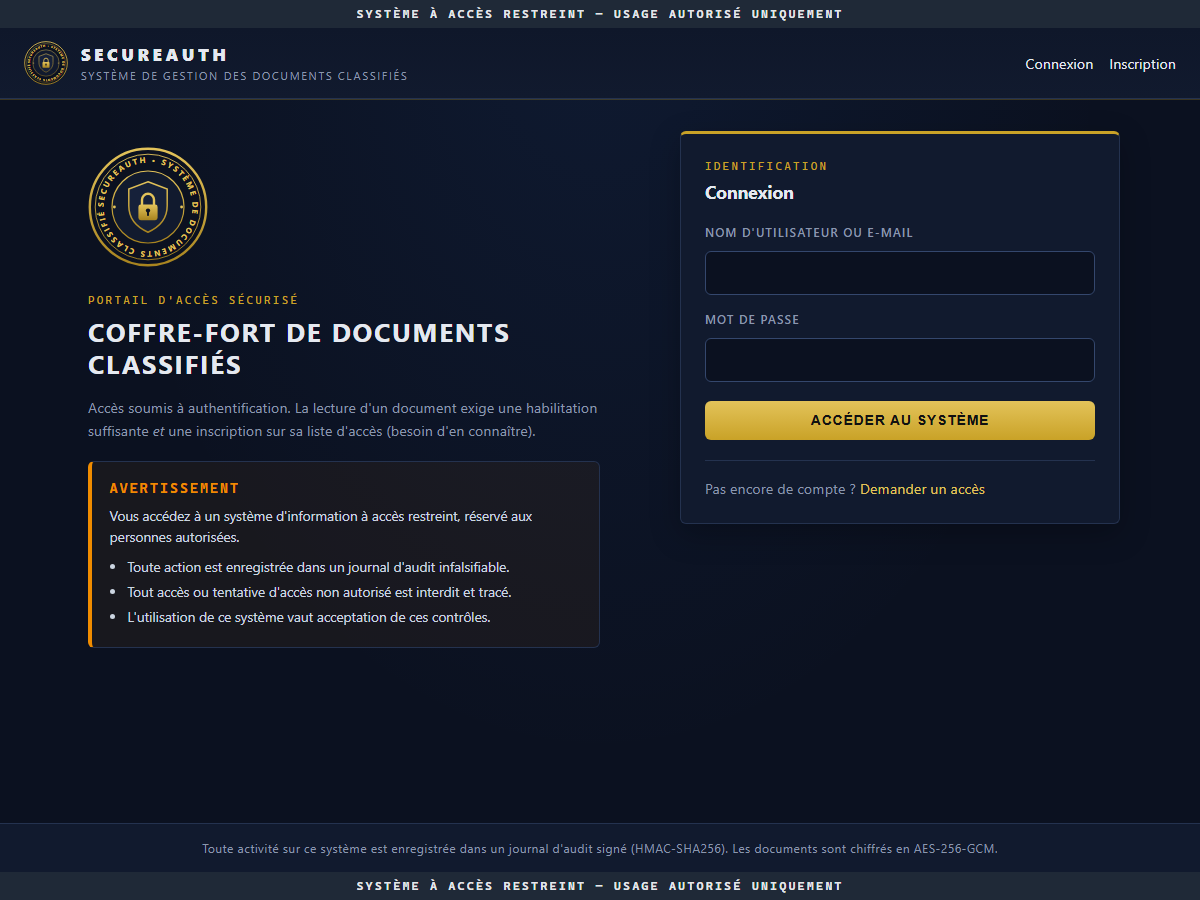
\includegraphics[width=0.88\linewidth]{img/captures/login.png}}
\caption{Page de connexion}
\end{figure}

\begin{figure}[H]
\centering
\fbox{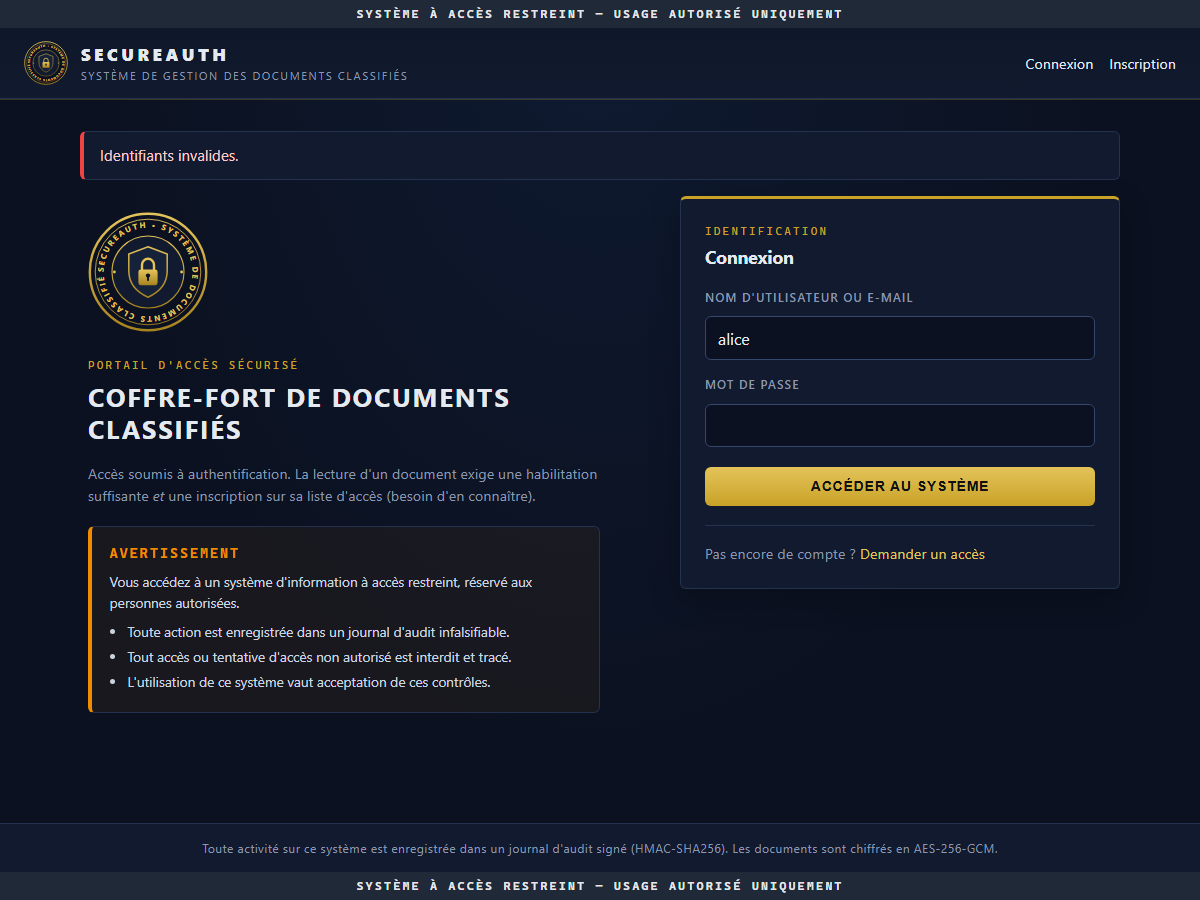
\includegraphics[width=0.88\linewidth]{img/captures/login-error.png}}
\caption{Échec de connexion : message unique}
\end{figure}

On peut se connecter avec le nom d'utilisateur ou l'adresse e-mail. Quand l'identifiant est inconnu, le compte désactivé ou le mot de passe faux, la page affiche toujours le même message, \og Identifiants invalides \fg, afin qu'un attaquant ne puisse pas deviner quels comptes existent. Le motif réel est conservé uniquement dans le journal d'audit.

\section{Tableau de Bord}

\begin{figure}[H]
\centering
\fbox{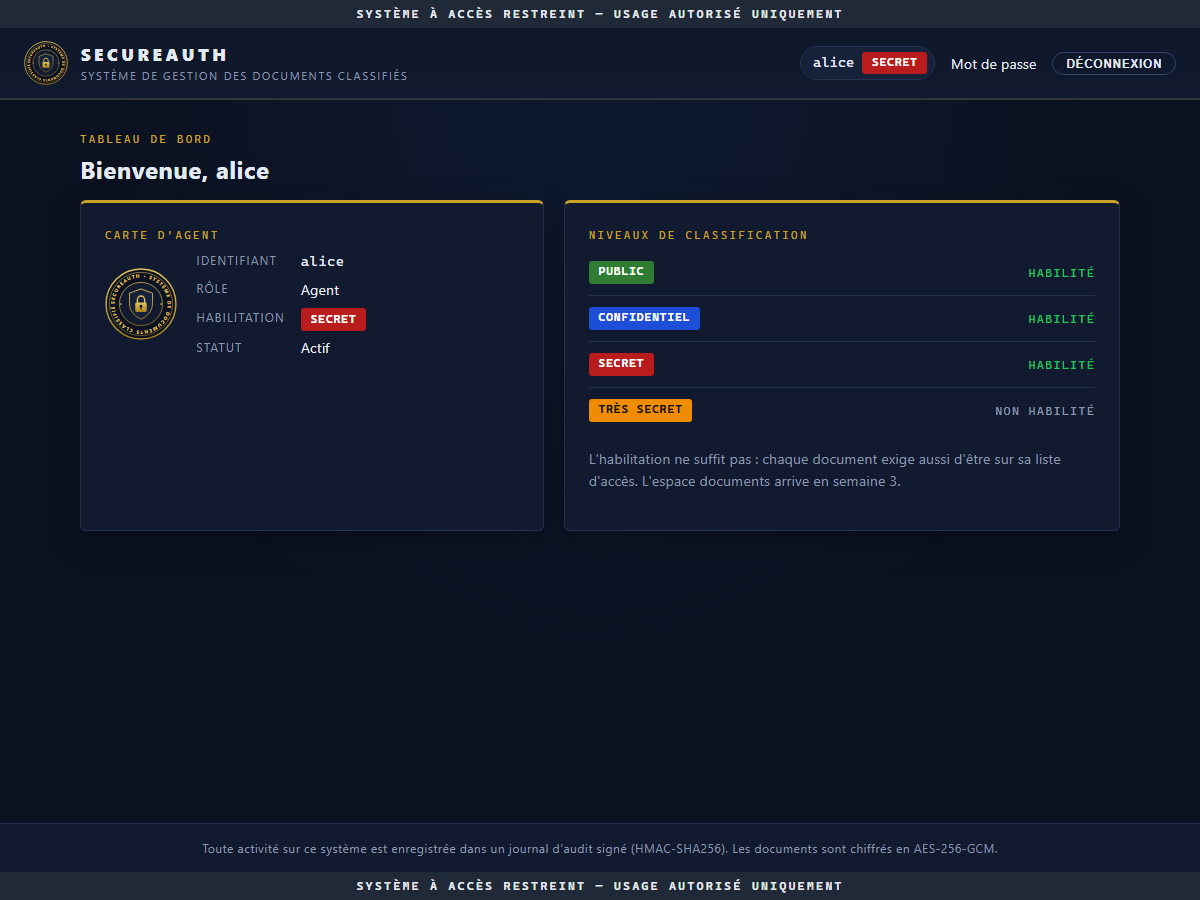
\includegraphics[width=0.88\linewidth]{img/captures/home.png}}
\caption{Tableau de bord d'un agent connecté}
\end{figure}

Après la connexion, l'agent voit sa carte d'identité (identifiant, rôle, habilitation, statut) et les quatre niveaux de classification, avec pour chacun la mention \og habilité \fg{} ou \og non habilité \fg. La page rappelle que l'habilitation ne suffit pas : il faut aussi figurer sur la liste d'accès du document. L'espace documents sera ajouté en semaine 3.

\section{Changement de Mot de Passe}

\begin{figure}[H]
\centering
\fbox{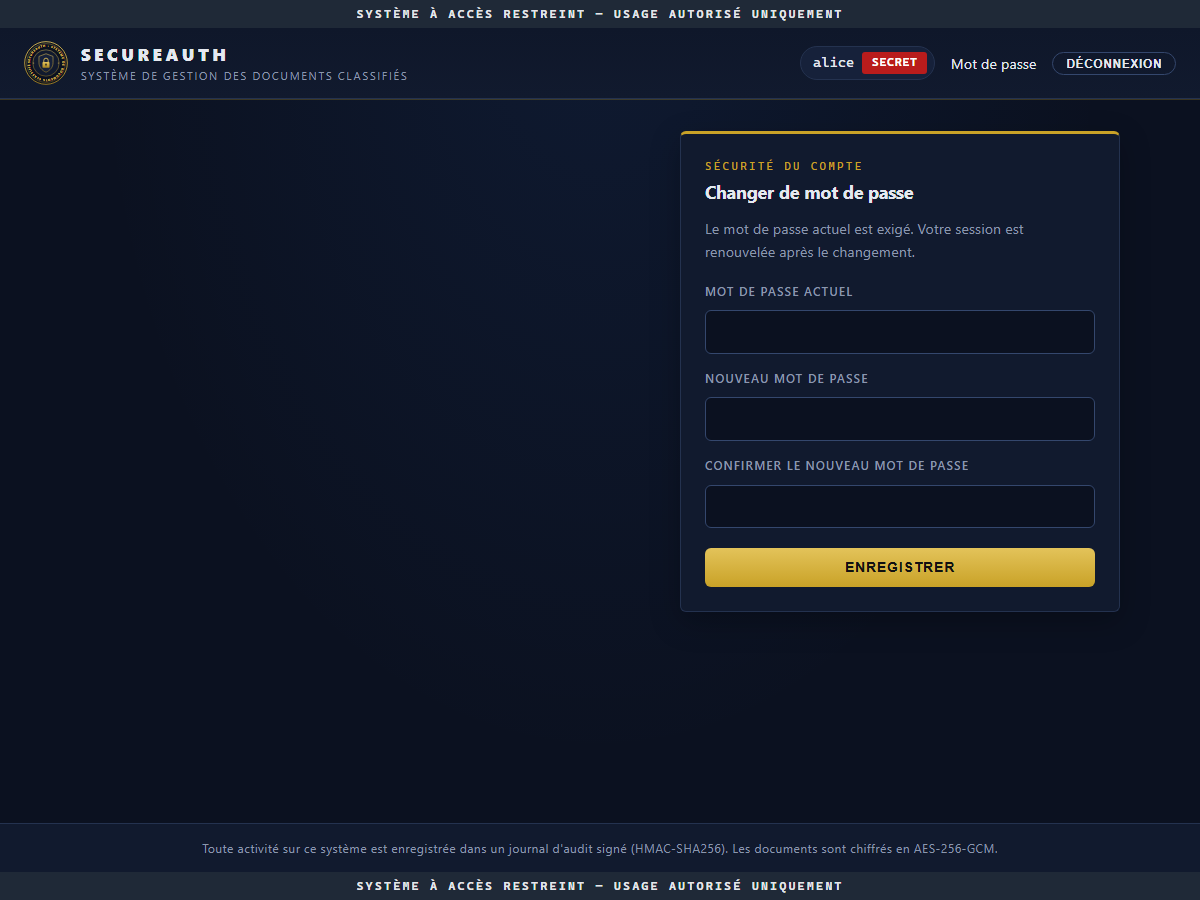
\includegraphics[width=0.88\linewidth]{img/captures/password.png}}
\caption{Changement de mot de passe}
\end{figure}

Pour changer son mot de passe, l'utilisateur doit saisir l'ancien. Le nouveau doit respecter la même politique qu'à l'inscription et être différent de l'ancien. Après le changement, l'identifiant de session est renouvelé : un cookie volé avant le changement ne sert plus à rien.

\section{Espace Documents}

\begin{figure}[H]
\centering
\fbox{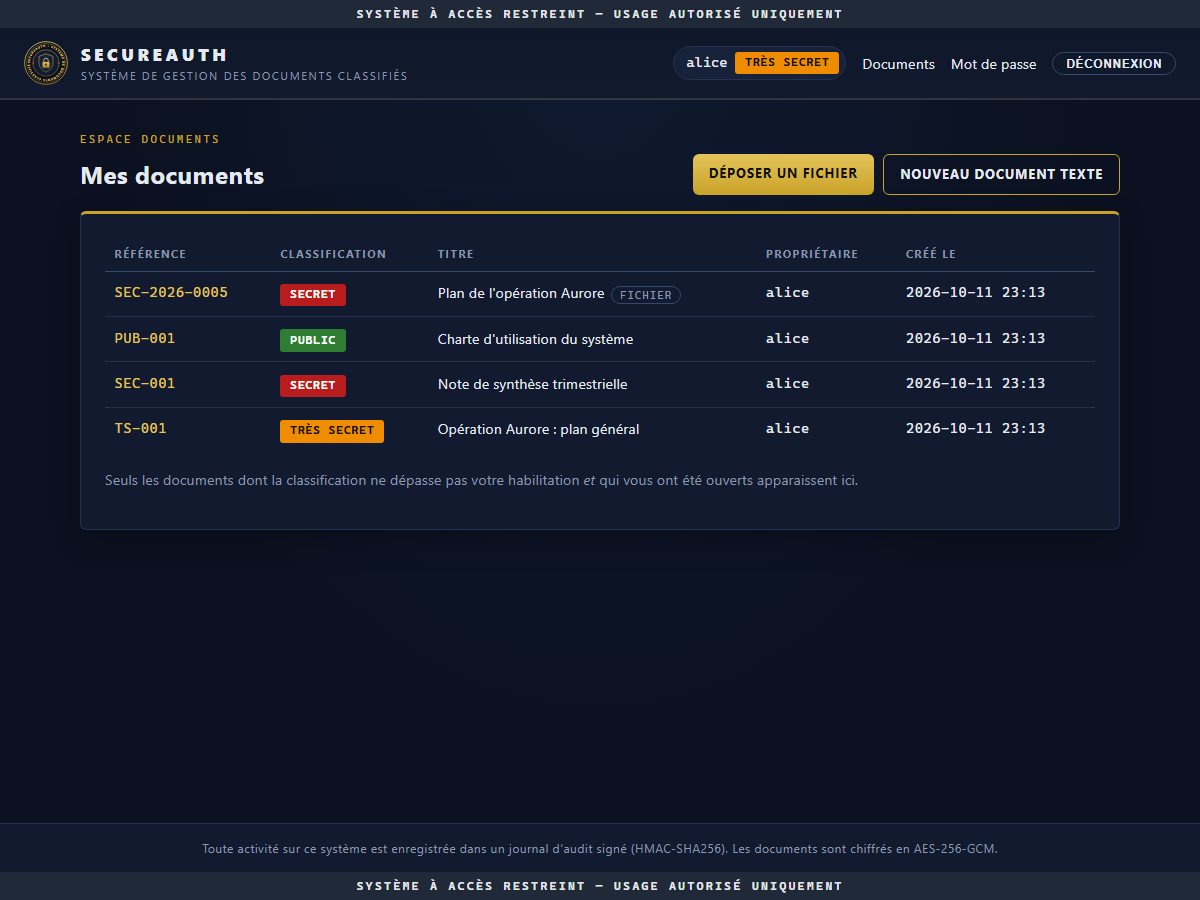
\includegraphics[width=0.84\linewidth]{img/captures/documents.png}}
\caption{Liste des documents lisibles par alice}
\end{figure}

La liste ne montre que les documents que l'agent peut lire : classification inférieure ou égale à son habilitation, et présence sur la liste d'accès. Le titre est déchiffré à l'affichage ; la référence, elle, est stockée en clair. Les adresses des documents utilisent un identifiant aléatoire (UUID) et jamais le numéro interne.

\begin{figure}[H]
\centering
\fbox{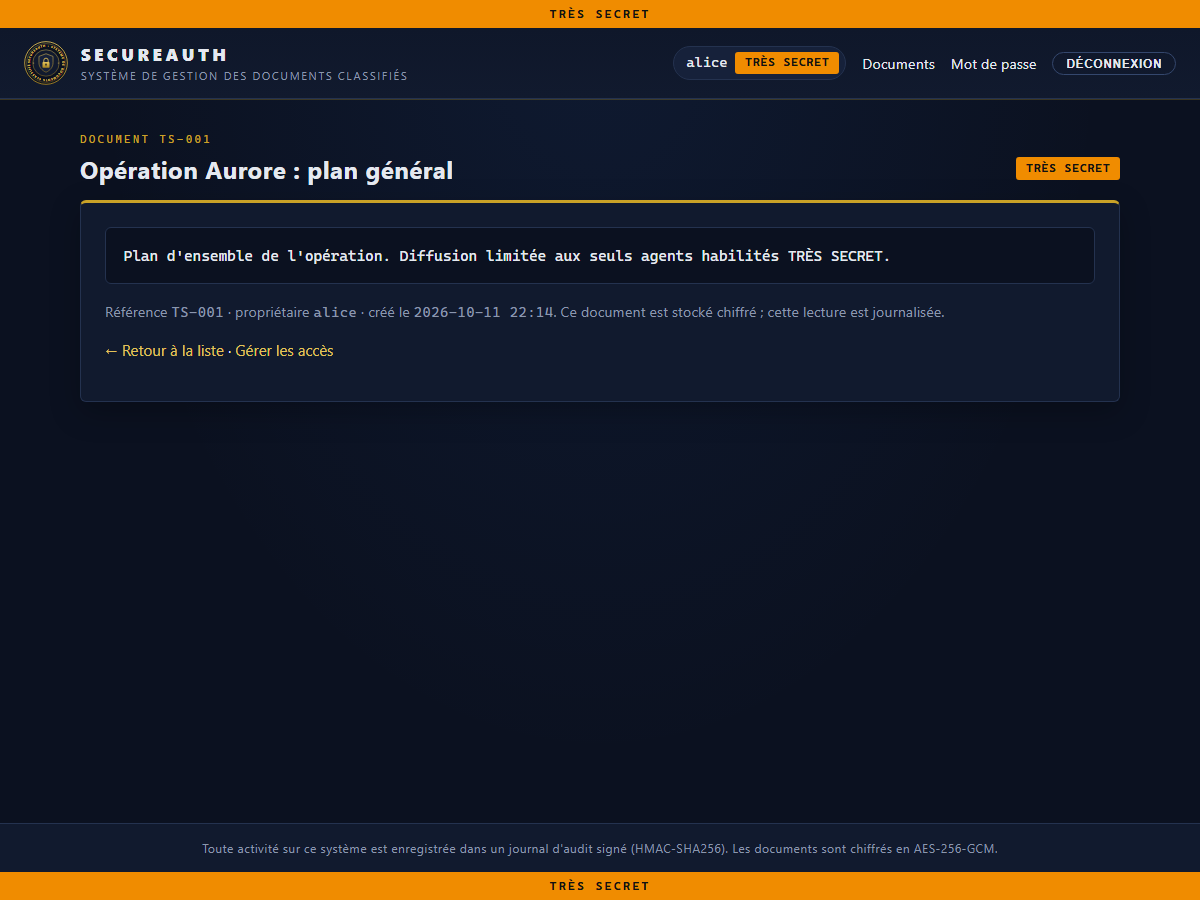
\includegraphics[width=0.84\linewidth]{img/captures/document-ts.png}}
\caption{Lecture d'un document TRÈS SECRET}
\end{figure}

À la lecture, le contenu est déchiffré puis affiché. Un bandeau de la couleur de la classification (orange pour TRÈS SECRET) encadre la page en haut et en bas. La lecture est inscrite dans le journal.

\begin{figure}[H]
\centering
\fbox{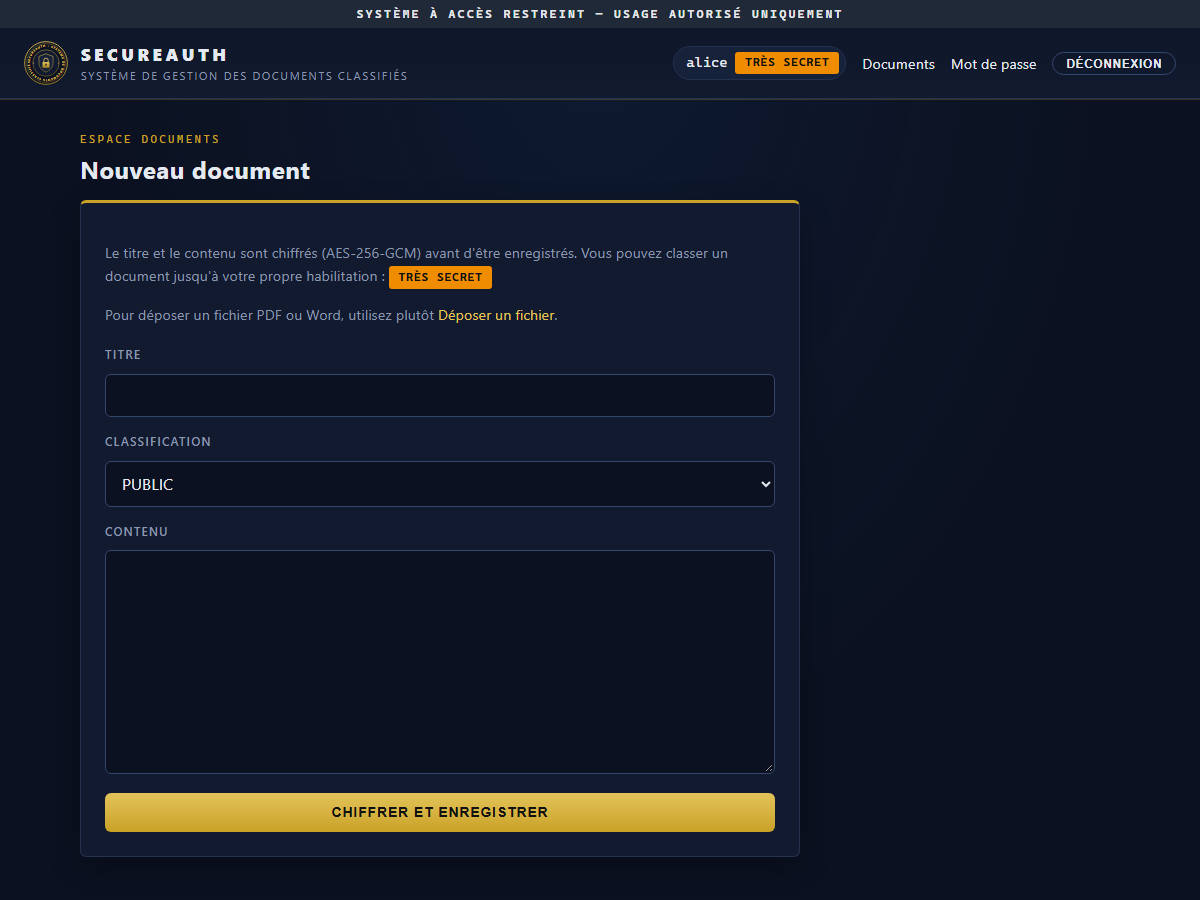
\includegraphics[width=0.84\linewidth]{img/captures/document-new.png}}
\caption{Création d'un document}
\end{figure}

Le formulaire de création ne propose que les niveaux jusqu'à l'habilitation de l'agent. Le serveur revérifie : un niveau forcé dans la requête est refusé et journalisé.

\begin{figure}[H]
\centering
\fbox{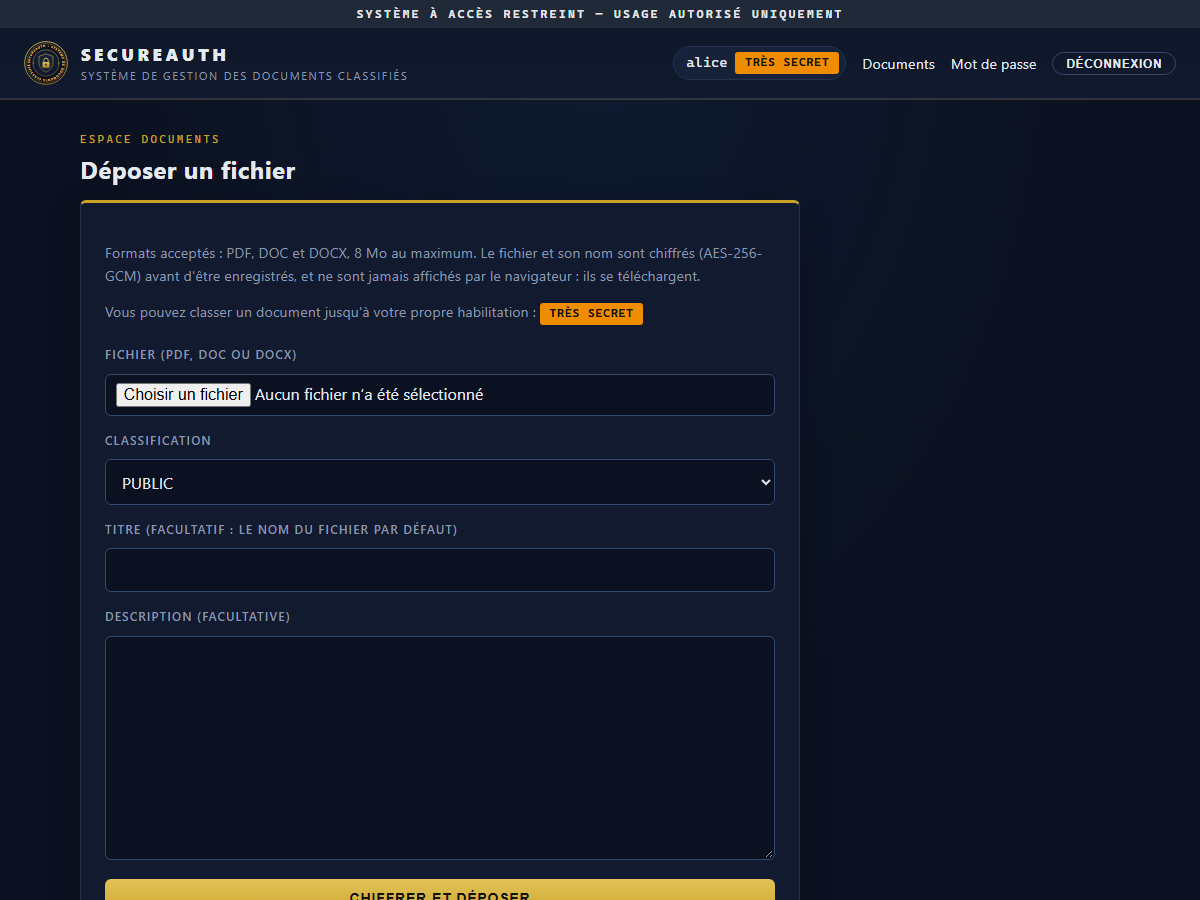
\includegraphics[width=0.84\linewidth]{img/captures/upload.png}}
\caption{Dépôt d'un fichier PDF, DOC ou DOCX}
\end{figure}

Le bouton \og Déposer un fichier \fg{} de la page des documents ouvre ce formulaire. L'agent choisit le fichier, sa classification (jusqu'à son habilitation), un titre facultatif et une description facultative. Trois contrôles s'enchaînent côté serveur : l'extension doit être \code{pdf}, \code{doc} ou \code{docx}, la taille ne dépasse pas huit mégaoctets, et le début du contenu doit correspondre au format annoncé (en-tête \code{\%PDF-} pour un PDF, signature OLE pour un DOC, archive contenant \code{word/} pour un DOCX). Un fichier \code{.pdf} qui n'est pas un PDF est donc refusé, et le refus est journalisé.

Le fichier est chiffré en AES-256-GCM avec son propre nonce, séparément du titre, de la description et du nom du fichier, qui sont chiffrés ensemble. Les données associées sont les mêmes que pour un document texte, avec un suffixe qui empêche de coller un fichier à la place des métadonnées, ou l'inverse.

\begin{figure}[H]
\centering
\fbox{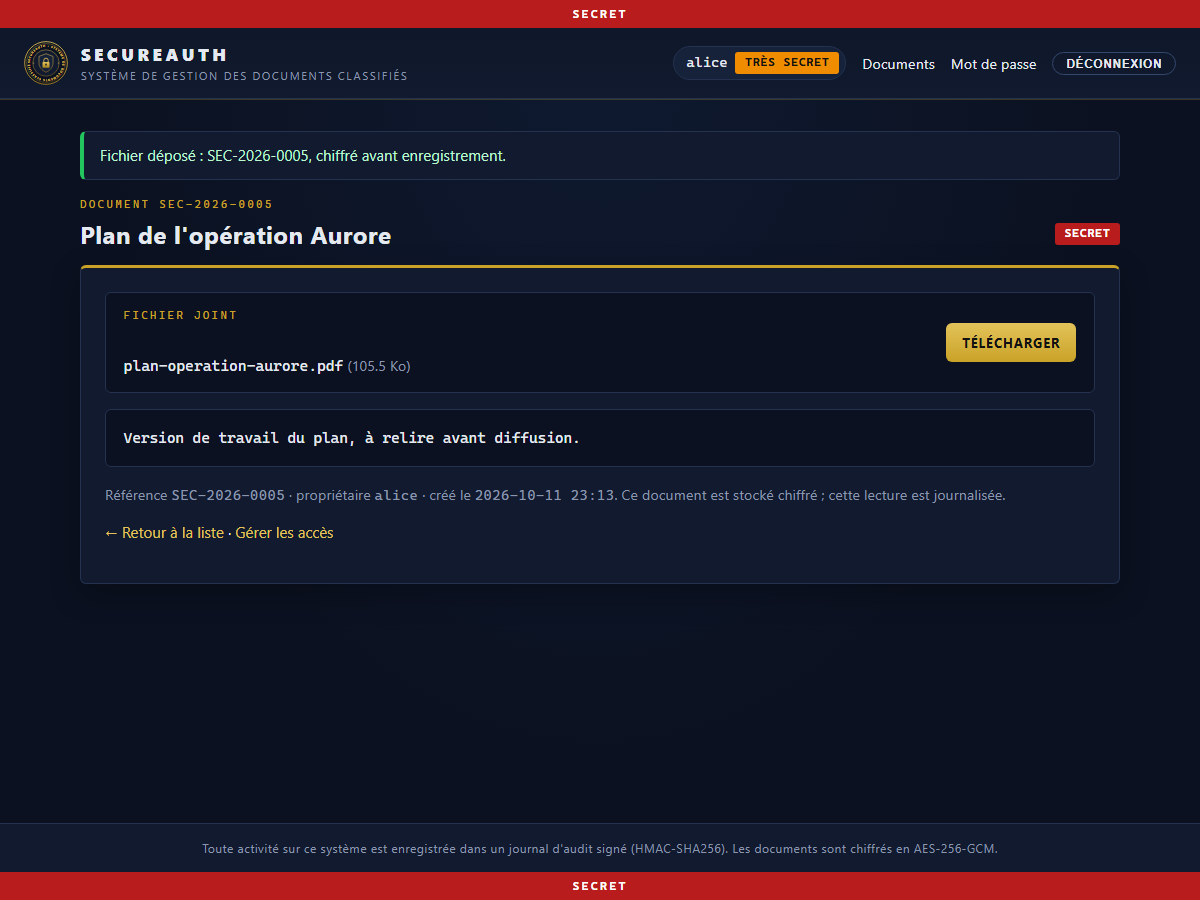
\includegraphics[width=0.84\linewidth]{img/captures/document-file.png}}
\caption{Fiche d'un document avec fichier joint}
\end{figure}

La fiche affiche le nom et la taille du fichier avec un bouton de téléchargement. Le fichier n'est jamais ouvert dans le navigateur : il est servi en pièce jointe, avec un type fixé par le serveur d'après l'extension et l'en-tête \code{X-Content-Type-Options: nosniff}. Le contrôle ne garantit que le format, pas l'innocuité : un PDF bien formé peut contenir du code actif, et aucun antivirus n'analyse les dépôts. Chaque téléchargement est inscrit dans le journal (événement \code{DOC\_DOWNLOAD}) sans le nom ni le contenu.

\begin{figure}[H]
\centering
\fbox{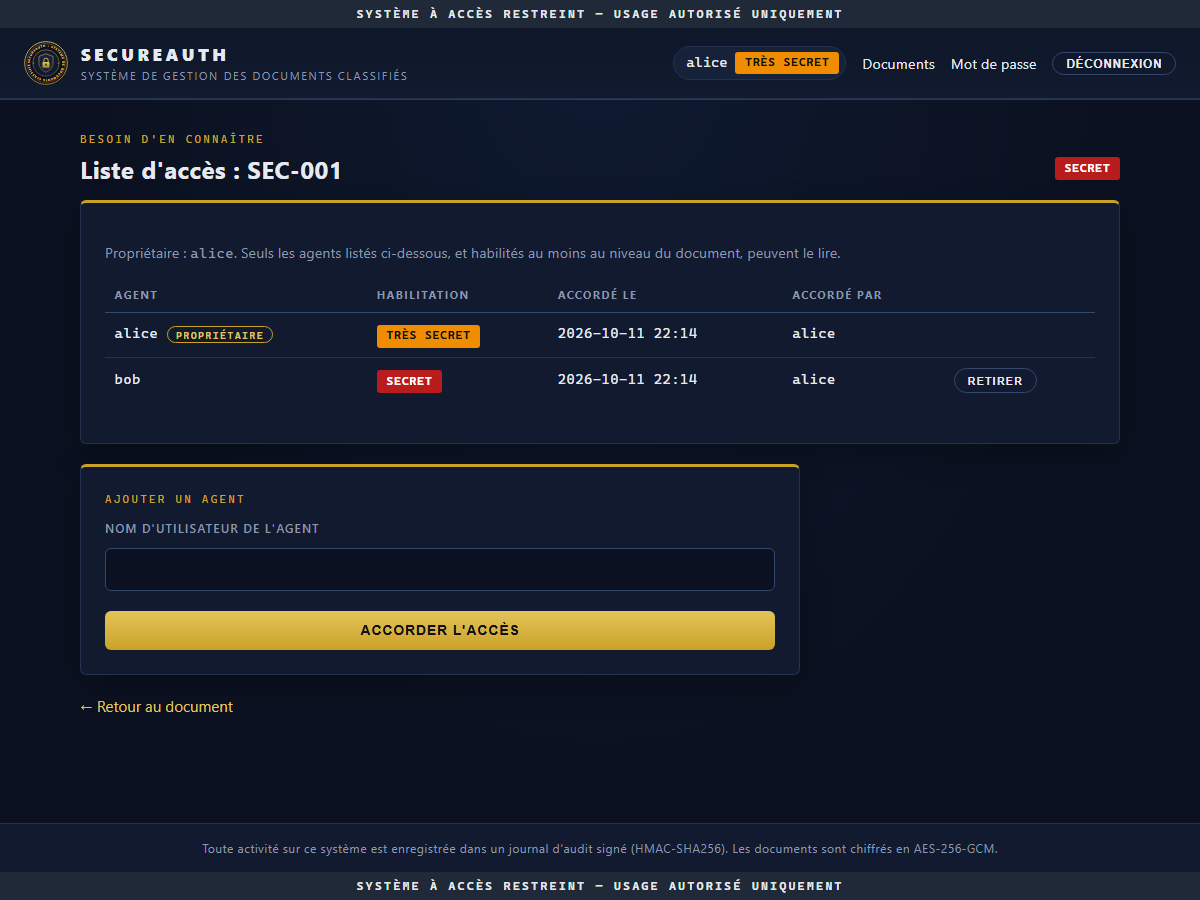
\includegraphics[width=0.84\linewidth]{img/captures/access.png}}
\caption{Liste d'accès d'un document (partage)}
\end{figure}

Le propriétaire (ou l'administrateur) ajoute ou retire des agents. Un agent insuffisamment habilité est refusé, et le propriétaire ne peut jamais perdre son propre accès.

\begin{figure}[H]
\centering
\fbox{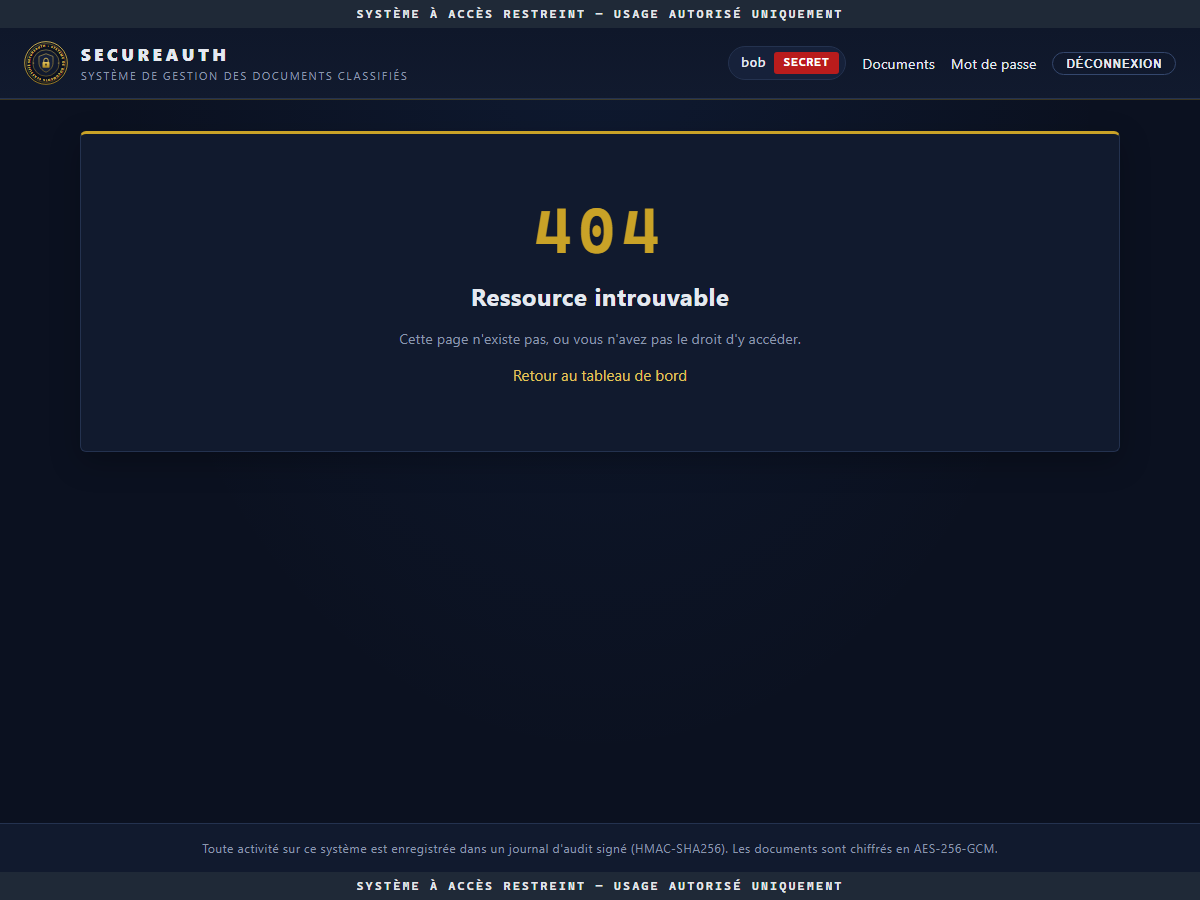
\includegraphics[width=0.84\linewidth]{img/captures/denied.png}}
\caption{Accès refusé : page 404 identique à un document inexistant}
\end{figure}

Quand bob (SECRET) force l'adresse de TS-001, il obtient la même page 404 que pour un document qui n'existe pas. Il ne peut donc pas savoir que ce document existe. Le refus, lui, est inscrit dans le journal.

\section{Espace Administration}

\begin{figure}[H]
\centering
\fbox{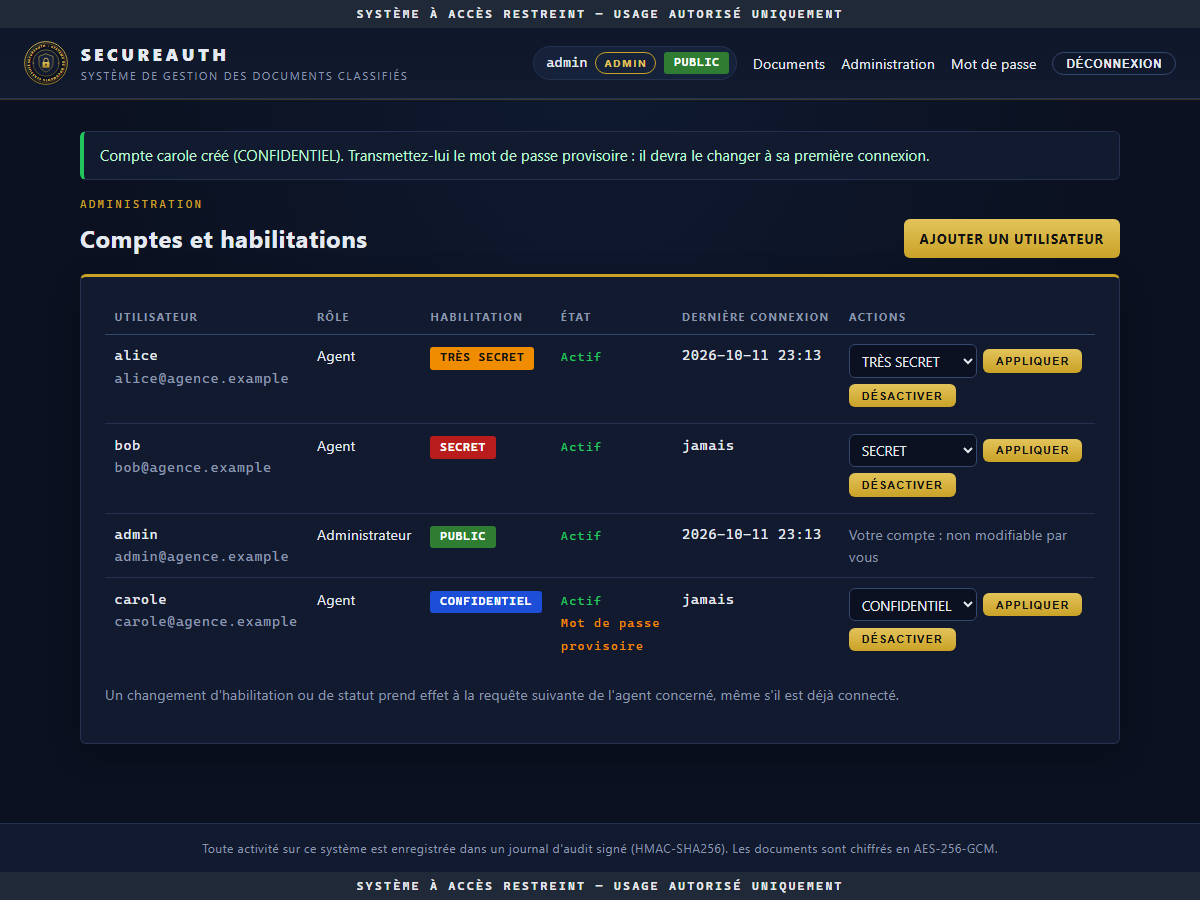
\includegraphics[width=0.84\linewidth]{img/captures/admin-users.png}}
\caption{Comptes et habilitations}
\end{figure}

L'administrateur voit les comptes, modifie une habilitation ou active et désactive un compte. Son propre compte n'est pas modifiable par lui. Un changement prend effet à la requête suivante de l'agent concerné, même s'il est déjà connecté.

\begin{figure}[H]
\centering
\fbox{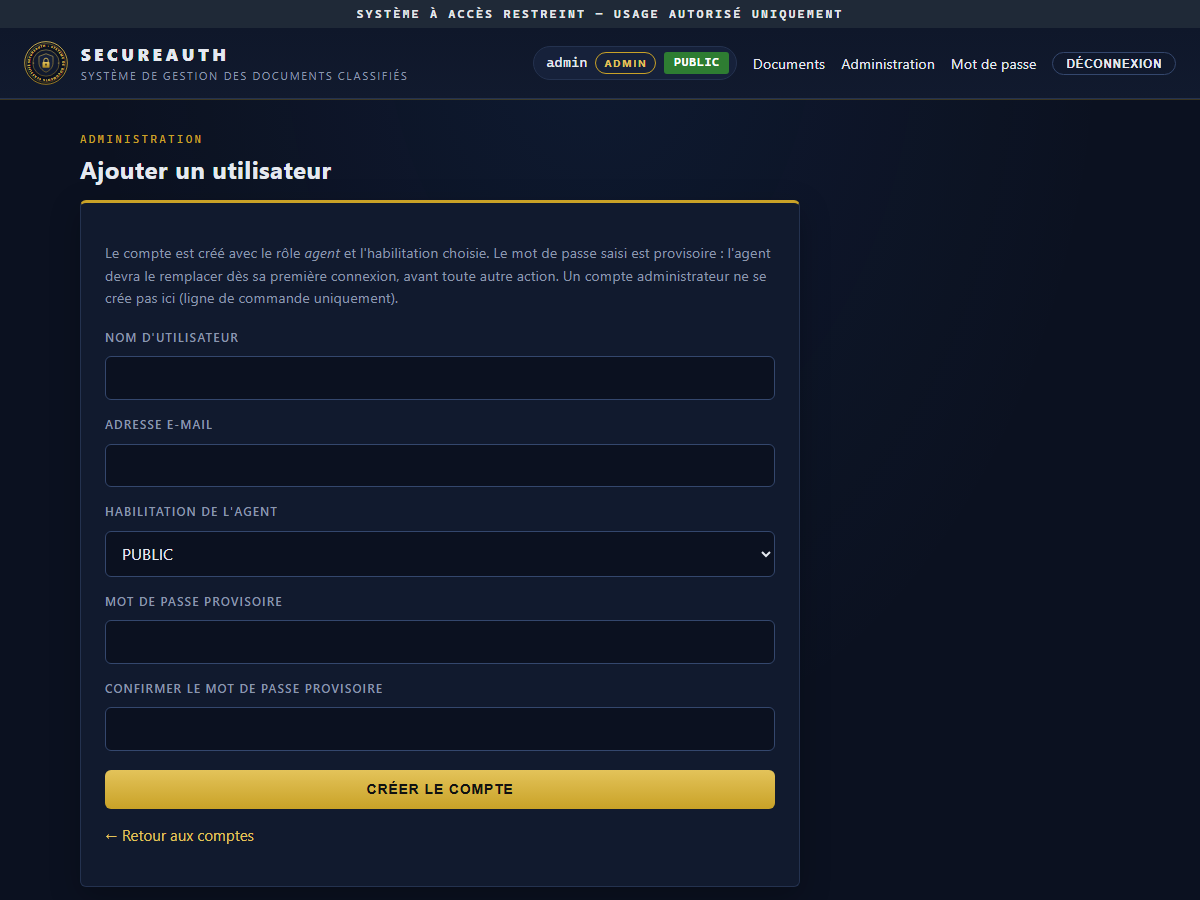
\includegraphics[width=0.84\linewidth]{img/captures/admin-user-new.png}}
\caption{Ajout d'un utilisateur par l'administrateur}
\end{figure}

Le bouton \og Ajouter un utilisateur \fg{} ouvre ce formulaire. L'administrateur saisit le nom, l'adresse e-mail, l'\textbf{habilitation} de l'agent (de PUBLIC à TRÈS SECRET) et un mot de passe provisoire, soumis à la même politique que le mot de passe d'une inscription. Le compte créé est toujours un compte agent : un administrateur ne se crée que par la ligne de commande, et un champ \og rôle \fg{} ajouté à la requête est ignoré. La création est inscrite dans le journal (\code{USER\_CREATE}) sans le mot de passe.

Le mot de passe provisoire est connu de l'administrateur, ce qui est contraire à l'idée qu'un mot de passe n'appartient qu'à son titulaire. Le compte porte donc un indicateur \og mot de passe provisoire \fg{} (visible dans la liste) : à sa première connexion, l'agent est redirigé vers le changement de mot de passe et ne peut rien faire d'autre, sauf se déconnecter, tant qu'il ne l'a pas remplacé.

\begin{figure}[H]
\centering
\fbox{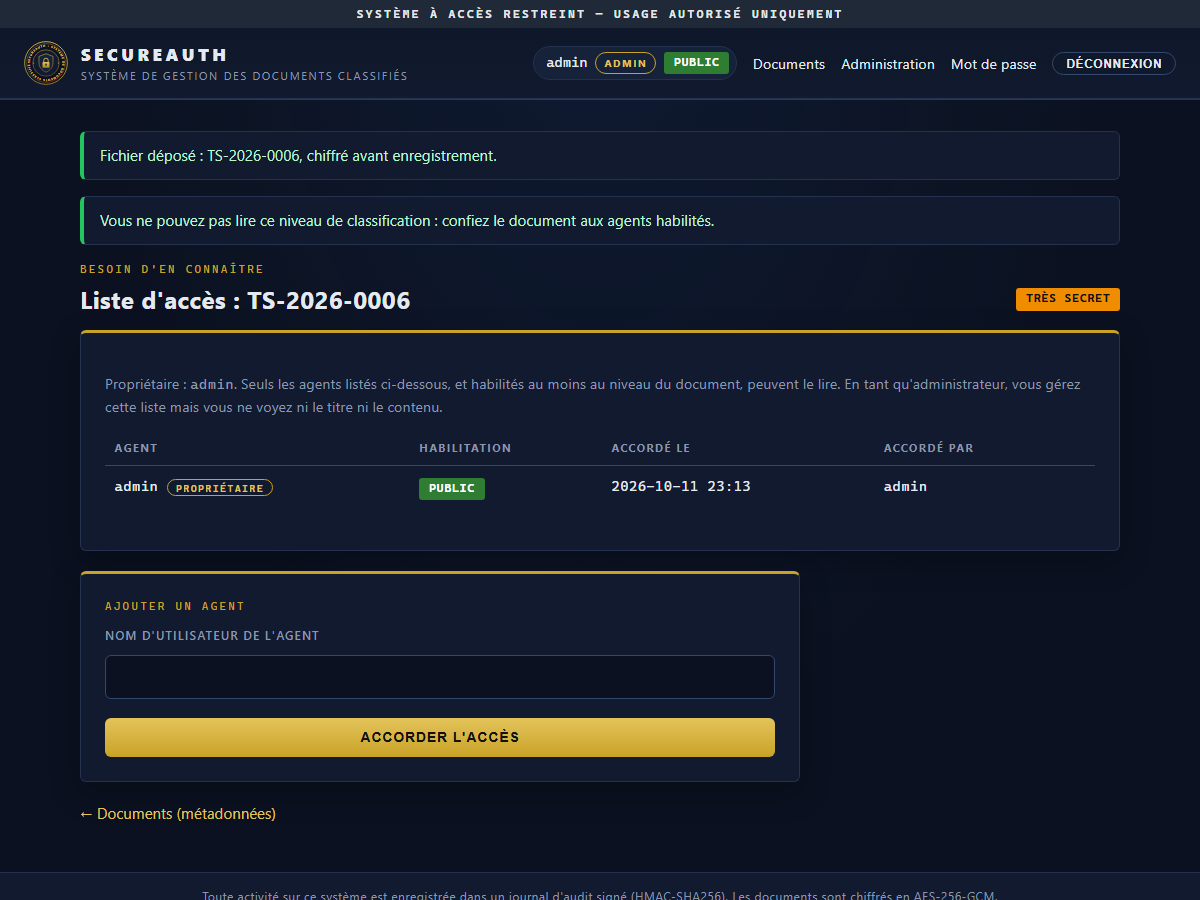
\includegraphics[width=0.84\linewidth]{img/captures/admin-upload-access.png}}
\caption{Dépôt par l'administrateur : classification TRÈS SECRET, puis partage}
\end{figure}

L'administrateur peut aussi déposer un document et il choisit sa classification à tous les niveaux, alors qu'un agent est limité à son habilitation. Son habilitation reste pourtant PUBLIC : il ne peut pas lire un document classé au-dessus (pas de lecture vers le haut, et le dépôt n'ajoute aucun droit). Après un dépôt à un niveau qu'il ne peut pas lire, il est donc conduit directement à la liste d'accès pour confier le document à des agents habilités. Un agent insuffisamment habilité est refusé, et l'administrateur ne peut pas s'ajouter lui-même.

\begin{figure}[H]
\centering
\fbox{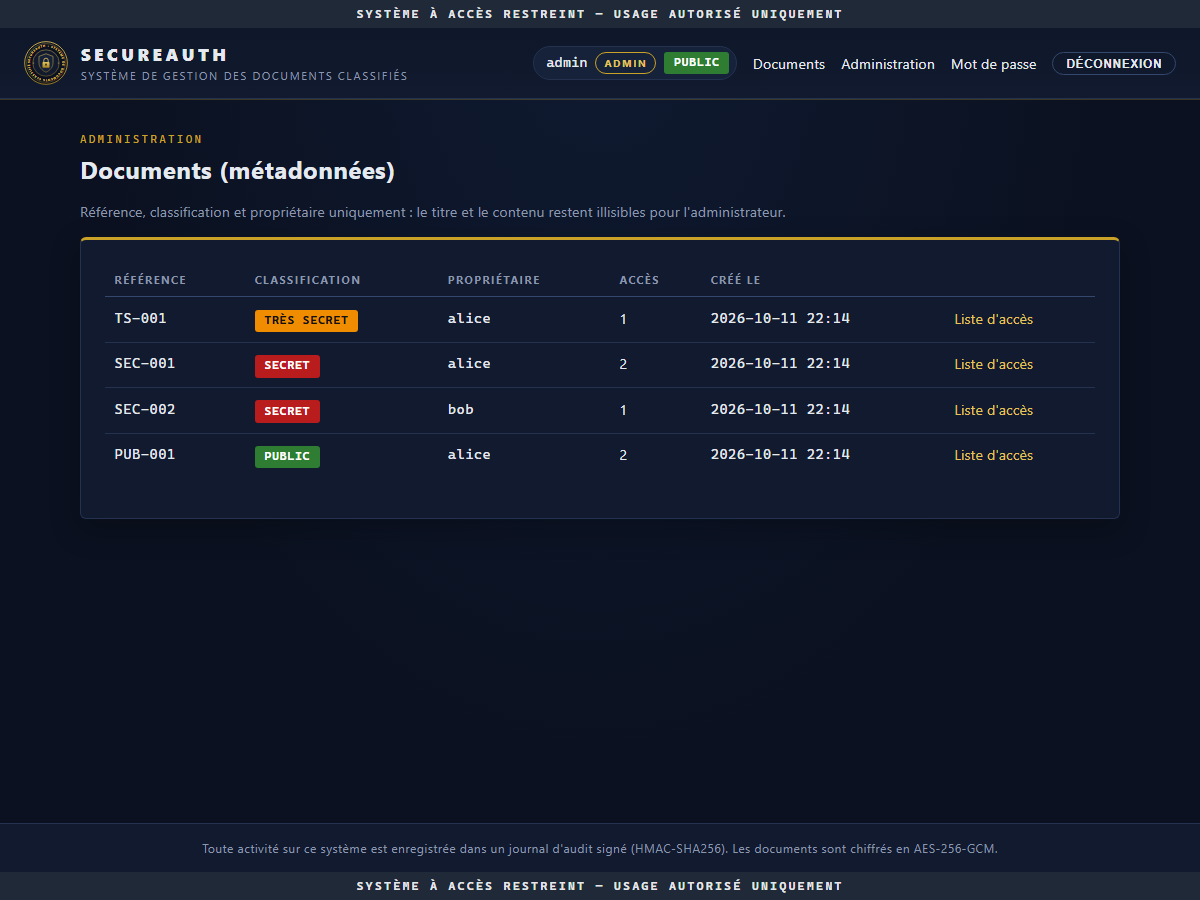
\includegraphics[width=0.84\linewidth]{img/captures/admin-documents.png}}
\caption{Documents : métadonnées uniquement}
\end{figure}

La page des documents donne la référence, la classification, le propriétaire et le nombre d'accès, mais jamais le titre ni le contenu.

\begin{figure}[H]
\centering
\fbox{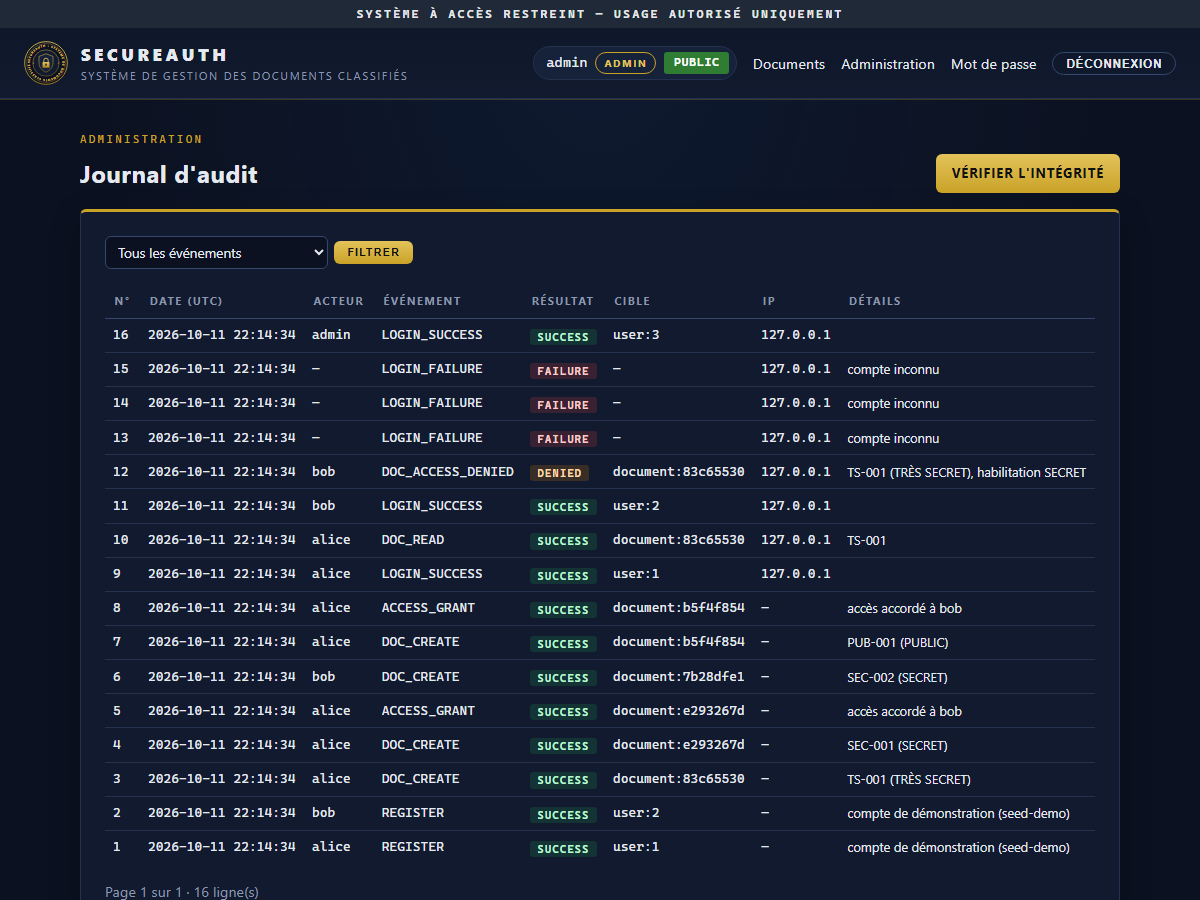
\includegraphics[width=0.84\linewidth]{img/captures/admin-audit.png}}
\caption{Journal d'audit}
\end{figure}

Le journal est paginé et filtrable par type d'événement. Chaque ligne indique l'acteur, l'événement, le résultat, la cible, l'adresse IP et un détail qui ne contient jamais de mot de passe, de contenu ni de clé.

\begin{figure}[H]
\centering
\fbox{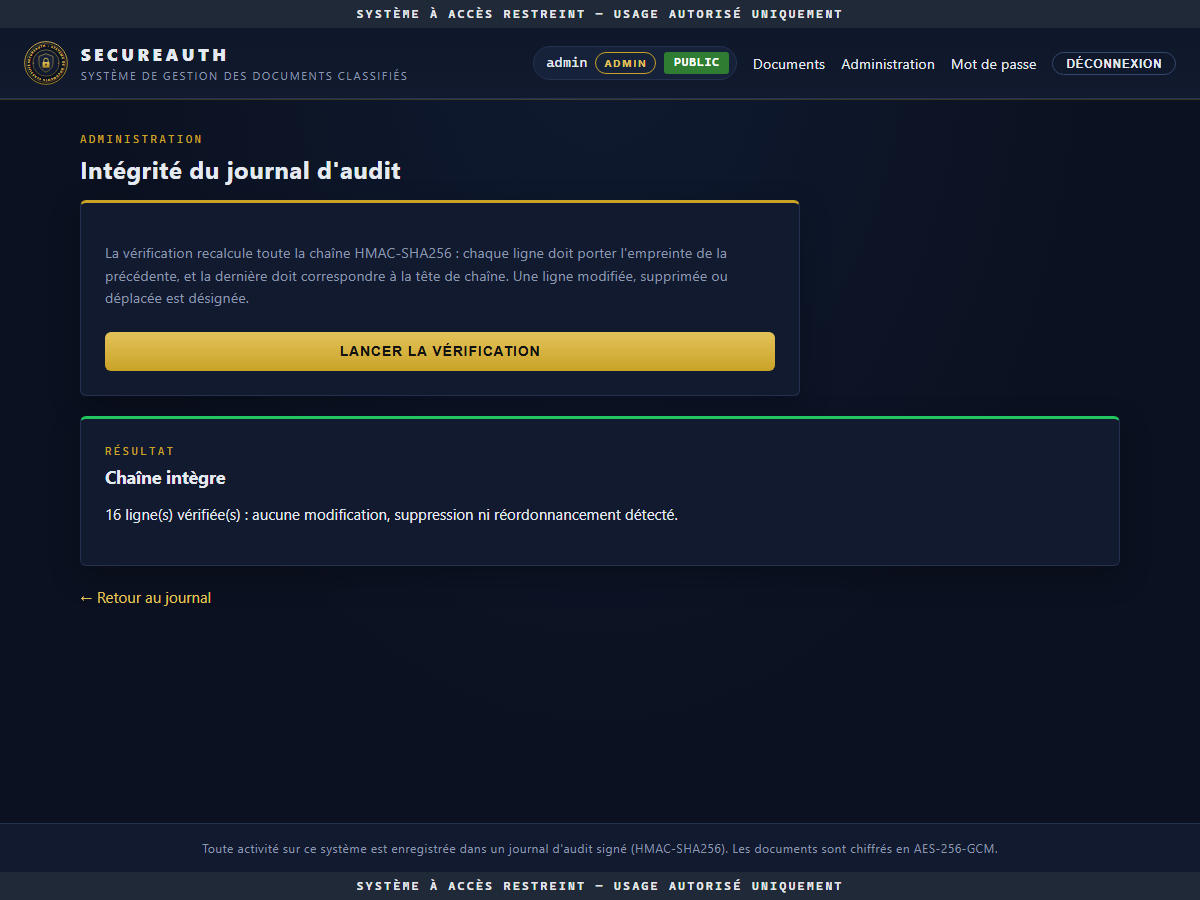
\includegraphics[width=0.84\linewidth]{img/captures/admin-verify-ok.png}}
\caption{Vérification du journal : chaîne intègre}
\end{figure}

\begin{figure}[H]
\centering
\fbox{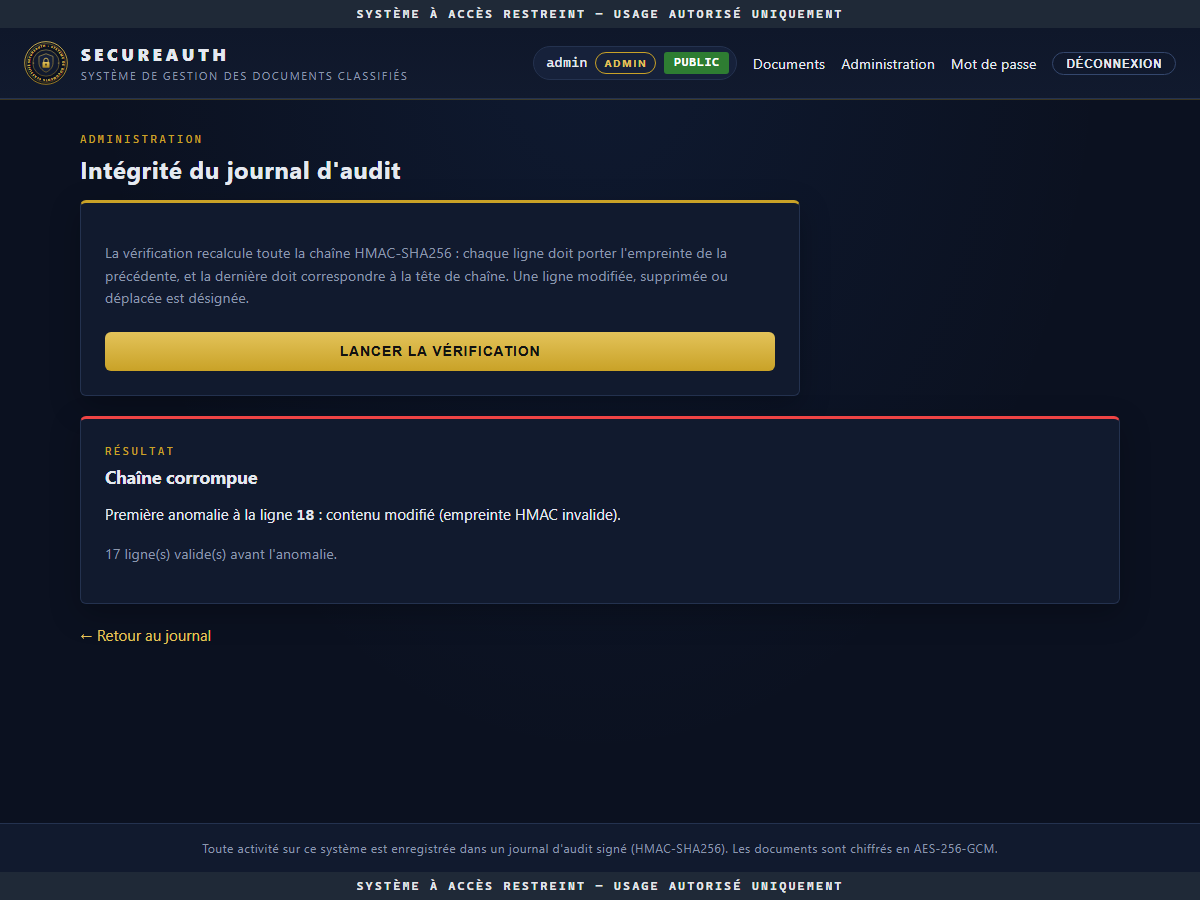
\includegraphics[width=0.84\linewidth]{img/captures/admin-verify-bad.png}}
\caption{Vérification du journal après modification d'une ligne en base}
\end{figure}

La vérification recalcule toute la chaîne HMAC. Quand une ligne a été modifiée directement en base, la page désigne la première ligne en cause (ici la ligne 18) et indique combien de lignes restaient valides avant elle.

% =====================================================
\chapter{Tests de Sécurité}
% =====================================================

\section{Méthode}

Le cahier des charges fixe vingt-cinq cas de test de sécurité, de T01 à T25. L'équipe en a ajouté cinq (T26 à T30) pour les fonctions apparues ensuite : comptes créés par l'administrateur, dépôt de fichiers, classification choisie par l'administrateur. Chacun est vérifié de deux façons.

\begin{itemize}
  \item \textbf{Des tests automatiques} (\code{pytest}), qui tournent sans conteneur avec une base en mémoire et un faux Redis. Ils couvrent les mots de passe, l'authentification, le verrouillage, les sessions, les règles d'accès, le chiffrement, les documents, le partage, l'administration, le journal d'audit, la limitation de débit, le jeu de démonstration et la configuration de l'infrastructure.
  \item \textbf{Un script contre l'application réellement déployée} (\code{live\_checks.py}) : HTTPS, Nginx, MariaDB et Redis en marche. Il rejoue ce qu'on ferait à la main avec \code{curl}, \code{openssl} et Burp Repeater : analyse du cookie, tentative de connexion en TLS 1.1, accès à un document d'un autre agent, modification d'une ligne du journal directement dans la base, rafale de connexions.
\end{itemize}

Les résultats complets sont dans \code{docs/tests-securite.md} et \code{docs/preuves/}. Les captures d'écran de Burp Suite restent à réaliser : le script envoie les mêmes requêtes, mais il ne les remplace pas dans le rapport final.

\section{Résultats}

\begin{longtable}{@{}l >{\raggedright\arraybackslash}p{5.6cm} >{\raggedright\arraybackslash}p{5.3cm} l@{}}
\caption{Les trente cas de test de sécurité (T26 à T30 : ajouts de l'équipe)}\\
\toprule
\textbf{Cas} & \textbf{Scénario} & \textbf{Résultat attendu} & \textbf{Résultat} \\
\midrule
\endfirsthead
\toprule
\textbf{Cas} & \textbf{Scénario} & \textbf{Résultat attendu} & \textbf{Résultat} \\
\midrule
\endhead
\bottomrule
\endfoot
T01 & Compte inexistant vs mauvais mot de passe & Même message, durée comparable & Conforme \\
T02 & 6 échecs consécutifs puis le bon mot de passe & Compte verrouillé 15 min, même message & Conforme \\
T03 & Injection SQL dans le formulaire (et les autres entrées) & Échec normal, aucune erreur SQL & Conforme \\
T04 & Drapeaux du cookie de session & Secure, HttpOnly, SameSite=Lax, préfixe \_\allowbreak{}\_\allowbreak{}Host- & Conforme \\
T05 & Identifiant avant / après connexion & Identifiant différent & Conforme \\
T06 & Rejouer un cookie après déconnexion & Redirection vers la connexion & Conforme \\
T07 & Inactivité supérieure à 30 minutes & Session expirée & Partiel \\
T08 & POST sans jeton & HTTP 400 & Conforme \\
T09 & Agent SECRET vers un document TRÈS SECRET & 404 + DOC\_\allowbreak{}ACCESS\_\allowbreak{}DENIED & Conforme \\
T10 & Habilitation suffisante mais hors liste d'accès & 404 & Conforme \\
T11 & IDOR : identifiant d'un autre document & 404 identique à un document inexistant & Conforme \\
T12 & L'administrateur tente de lire un document & 404 & Conforme \\
T13 & L'administrateur s'attribue un accès ou modifie sa propre habilitation & Refus + ADMIN\_\allowbreak{}SELF\_\allowbreak{}MODIFY\_\allowbreak{}DENIED & Conforme \\
T14 & Un agent appelle une route /admin/* & 403 & Conforme \\
T15 & Habilitation abaissée après attribution & Accès perdu immédiatement & Conforme \\
T16 & Création au-dessus de son habilitation (champ modifié) & Refus & Conforme \\
T17 & Classification modifiée directement en base & Déchiffrement impossible + INTEGRITY\_\allowbreak{}FAILURE & Conforme \\
T18 & Lecture des documents directement en base & Uniquement du binaire illisible & Conforme \\
T19 & Ligne du journal modifiée en base & Ligne signalée & Conforme \\
T20 & Ligne du journal supprimée (milieu ou fin) & Rupture détectée & Conforme \\
T21 & Balise de script dans un titre de document & Affichée comme texte, bloquée par la CSP & Conforme \\
T22 & Connexion en TLS 1.1 & Refusée & Conforme \\
T23 & En-têtes de sécurité & Tous présents & Conforme \\
T24 & Accès direct aux ports 3306 et 6379 & Injoignables depuis l'hôte & Conforme \\
T25 & Rafale de connexions & HTTP 429 après le seuil & Conforme \\
T26 & L'administrateur ajoute un agent ; l'agent ouvre le formulaire ; première connexion & Agent refusé (403) ; compte créé avec mot de passe provisoire ; changement imposé ; USER\_\allowbreak{}CREATE sans mot de passe & Conforme \\
T27 & Dépôt d'un PDF de 3 Mo puis lecture directe de la colonne en base & Binaire illisible, ni contenu ni nom en clair ; téléchargement identique en pièce jointe & Conforme \\
T28 & Téléchargement hors liste d'accès, après partage, puis classification modifiée en base & 404 + DOC\_\allowbreak{}ACCESS\_\allowbreak{}DENIED ; 200 après partage ; 500 + INTEGRITY\_\allowbreak{}FAILURE après falsification & Conforme \\
T29 & Faux PDF, exécutable, page HTML, fichier de 11 Mo, corps de 3 Mo sur une autre page & 400 pour les fichiers invalides, 413 pour les envois trop gros, rien d'enregistré & Conforme \\
T30 & L'administrateur dépose un document TRÈS SECRET puis tente de le lire & Dépôt accepté, redirection vers le partage, lecture et téléchargement refusés (404), partage seulement aux agents habilités & Conforme \\

\end{longtable}

Vingt-neuf cas sur trente sont conformes. Le cas T07 (inactivité de plus de trente minutes) est partiel : la durée absolue de huit heures est testée, et le cookie ainsi que la clé Redis expirent bien après trente minutes, mais l'attente réelle de trente minutes n'a pas été rejouée. Le cas T20 (suppression d'une ligne du journal) est démontré par les tests automatiques seulement, pour ne pas détruire la chaîne du journal de la base réelle : une ligne signée supprimée ne peut pas être reconstituée.

\section{Défauts découverts et corrigés}

Les tests contre les vrais services ont fait apparaître des défauts que les tests automatiques ne pouvaient pas voir.

\begin{itemize}
  \item Le certificat du serveur n'avait pas d'identifiant de clé de l'autorité (\emph{Authority Key Identifier}) : les clients stricts, comme Python 3.14, le refusaient. Le script de génération de la mini-PKI ajoute maintenant ces identifiants, et le certificat a été réémis avec la même clé.
  \item La première limite de débit de Nginx comptait aussi les pages affichées : ouvrir le formulaire de connexion consommait le quota. Seules les requêtes \code{POST} sont désormais comptées.
  \item Le verrouillage du compte, prévu en semaine 2, n'était pas encore codé : le champ existait mais aucune route ne l'utilisait. Il est implémenté et testé.
  \item La création d'un document échouait sur MariaDB (\emph{Data too long for column}) alors qu'elle passait avec SQLite : la référence provisoire était plus longue que la colonne. La base en mémoire des tests automatiques n'applique pas les longueurs, seul le test contre la vraie base l'a révélé ; la référence est raccourcie et deux tests de non-régression ont été ajoutés.
\end{itemize}

\begin{sloppypar}
Une observation sur l'environnement : sur la machine de développement, \code{localhost:3306} répond, car c'est le MariaDB de XAMPP et non le conteneur. La preuve que Docker ne publie rien est donc la colonne des ports de \code{docker compose ps}, pas un test de connexion depuis l'hôte.
\end{sloppypar}

\section{Durcissement}

En semaine 5, plusieurs protections ont été ajoutées :
\begin{itemize}
  \item limitation de débit par adresse IP, à deux niveaux (Flask-Limiter avec compteurs dans Redis, et \code{limit\_req} dans Nginx) ; au-delà du seuil, la réponse est HTTP 429 ;
  \item HSTS avec une durée courte de cinq minutes, pour ne pas piéger \code{localhost} ;
  \item conteneur applicatif en lecture seule, sans capacités Linux et sans élévation de privilèges ;
  \item en-tête \code{Cache-Control: no-store} sur toute page affichée à un agent connecté, pour que le bouton \og Précédent \fg{} ne rouvre pas un document après la déconnexion ;
  \item des tests d'infrastructure qui échouent si la configuration livrée s'affaiblit ;
  \item pour le dépôt de fichiers : liste blanche d'extensions, contrôle de la signature du contenu, taille limitée à huit mégaoctets, nom de fichier nettoyé, téléchargement en pièce jointe uniquement. La limite de corps de requête de Nginx reste à deux mégaoctets partout, sauf sur la seule adresse de dépôt (dix mégaoctets), et l'application relève sa propre limite pour cette seule page.
\end{itemize}

% =====================================================
\chapter{Conclusion et Perspectives}
% =====================================================

\section{Bilan du Projet}

Les six semaines du projet sont réalisées. L'infrastructure fonctionne en quatre conteneurs avec un réseau interne et du TLS signé par une mini-autorité locale. L'authentification est complète : inscription, connexion avec un message d'erreur unique, verrouillage du compte après cinq échecs, sessions côté serveur renouvelées à la connexion, changement de mot de passe. L'autorisation repose sur un module unique qui applique la lecture sans montée de niveau, le besoin d'en connaître et la séparation des rôles. Les documents sont chiffrés en AES-256-GCM avec des données associées qui scellent leur classification. Le journal d'audit est chaîné par HMAC-SHA256 et vérifiable depuis la ligne de commande comme depuis l'interface. L'administrateur peut ouvrir des comptes agents avec l'habilitation de son choix (mot de passe provisoire à changer immédiatement), et les agents peuvent déposer des fichiers PDF, DOC et DOCX, chiffrés à part et téléchargeables seulement par ceux qui ont le droit de les lire. Plus de trois cents tests automatiques passent, et les attaques ont été rejouées contre l'application déployée.

\textbf{Points forts :}
\begin{itemize}
  \item les mots de passe sont protégés par Argon2id et jamais conservés en clair ;
  \item un document interdit répond par la même page 404 qu'un document inexistant ;
  \item l'administrateur gère les comptes mais ne peut lire aucun document, ni modifier ses propres droits ;
  \item changer la classification d'un document directement en base le rend illisible au lieu de le livrer ;
  \item le rôle et l'habilitation sont relus en base à chaque requête : une désactivation ou une baisse d'habilitation prend effet immédiatement ;
  \item toute modification, suppression ou permutation d'une ligne du journal est détectée, et la page d'administration désigne la première ligne en cause ;
  \item l'application refuse de démarrer si une clé est absente, mal formée ou si les deux clés sont identiques ;
  \item un fichier déposé n'est jamais en clair en base ni dans le journal, son format est vérifié sur son contenu et pas seulement sur son nom, et l'administrateur qui choisit la classification d'un dépôt ne gagne aucun droit de lecture.
\end{itemize}

\textbf{Ce qui reste à faire :} les captures d'écran de Burp Suite pour le rapport final, l'attente réelle de trente minutes pour le cas T07, et les points listés dans les perspectives.

\section{Leçons Apprises}

\begin{itemize}
  \item \textbf{Les détails de sécurité se cachent dans le temps de réponse.} Pour ne pas révéler l'existence d'un compte, il faut calculer l'empreinte Argon2id même quand le compte n'existe pas, et le faire avant le test d'unicité à l'inscription. La mesure sur le service réel donne environ 125 ms pour un compte inconnu et 115 ms pour un mauvais mot de passe.
  \item \textbf{Une bibliothèque peut ne rien faire sans prévenir.} Avec Flask-Session, la régénération d'une session vide ne fait rien : il faut écrire l'identifiant de l'utilisateur dans la session avant de la régénérer, sinon la protection contre la fixation de session est inopérante.
  \item \textbf{Une signature est exigeante.} Le journal d'audit est déclaré corrompu si la date relue diffère d'une microseconde de la date signée : la colonne doit donc stocker les microsecondes.
  \item \textbf{Tester en vrai ne donne pas les mêmes résultats que tester en mémoire.} Le certificat sans identifiant d'autorité, la limite Nginx qui comptait les GET et le port 3306 de XAMPP n'apparaissent qu'avec les vrais services.
  \item \textbf{Un contexte partagé peut masquer des erreurs.} Flask-WTF garde le jeton CSRF dans un objet lié au contexte d'application : si plusieurs clients de test partagent ce contexte, le deuxième échoue pour une raison qui n'existe pas en production. Les tests donnent donc un contexte à chaque requête.
  \item \textbf{L'environnement de développement compte.} Sous Windows, Apache de XAMPP occupait déjà les ports 80 et 443 ; \code{curl} est un alias dans PowerShell (il faut écrire \code{curl.exe}) ; et la vérification de révocation du certificat échoue car l'autorité locale n'a pas de liste de révocation.
\end{itemize}

\section{Perspectives d'Évolution}

\begin{itemize}
  \item authentification multifacteur ;
  \item analyse antivirus des fichiers déposés (par exemple avec ClamAV dans un conteneur dédié) et conversion en un format sans code actif ;
  \item réinitialisation du mot de passe par lien à usage unique, pour que l'administrateur n'ait plus à connaître de mot de passe provisoire ;
  \item rotation des clés et stockage dans un coffre-fort de secrets ou un module matériel (HSM) ;
  \item règle \emph{no write down} du modèle Bell-LaPadula et reclassification contrôlée des documents ;
  \item protection des habilitations par un tag HMAC, pour détecter une modification directe en base ;
  \item liste de révocation (CRL ou OCSP) pour l'autorité de certification ;
  \item déverrouillage d'un compte par l'administrateur et notification de l'utilisateur ;
  \item HSTS d'un an et certificat émis par une autorité reconnue, pour une mise en production ;
  \item migrations de schéma (Alembic) et API publique, aujourd'hui hors périmètre.
\end{itemize}

\section{Conclusion Générale}

SecureAuth part d'une idée simple : une application sécurisée ne repose jamais sur une seule protection. Ici, l'authentification identifie l'utilisateur, l'autorisation décide de ce qu'il peut lire, la cryptographie protège les documents même si la base est lue directement, et le journal signé permet de prouver ce qui s'est passé.

Le projet montre aussi qu'une protection n'existe vraiment que si on l'a attaquée. Les tests automatiques ont fixé le comportement attendu, puis les mêmes attaques rejouées contre les services en marche ont révélé des défauts de configuration que le code seul ne montrait pas. Les limites restantes sont connues et écrites : un attaquant qui modifie directement l'habilitation d'un compte en base n'est pas détecté, la détention de la clé HMAC permettrait de refaire une chaîne valide, et l'autorité de certification locale ne peut pas révoquer un certificat. Chaque décision de sécurité du projet peut ainsi être justifiée et démontrée par une preuve, ce qui était l'objectif du module.

% =====================================================
\appendix
\chapter{Glossaire}
% =====================================================

\begin{description}
  \item[AAD] Données associées : informations non chiffrées mais protégées par AES-GCM ; si on les modifie, le déchiffrement échoue.
  \item[AES-256-GCM] Chiffrement symétrique authentifié : il garantit à la fois la confidentialité et l'intégrité.
  \item[Argon2id] Fonction de hachage de mots de passe, volontairement lente et gourmande en mémoire pour résister à la force brute.
  \item[Bell-LaPadula] Modèle de confidentialité : pas de lecture vers le haut, pas d'écriture vers le bas.
  \item[Besoin d'en connaître] Principe selon lequel l'habilitation ne suffit pas : il faut une autorisation explicite pour chaque document.
  \item[Classification] Niveau de sensibilité d'un document : PUBLIC, CONFIDENTIEL, SECRET ou TRÈS SECRET.
  \item[CSRF] Attaque qui fait exécuter une action à un utilisateur connecté depuis un autre site.
  \item[Fixation de session] Attaque qui impose à la victime un identifiant de session connu de l'attaquant.
  \item[Habilitation] Niveau maximal de classification qu'un utilisateur est autorisé à lire.
  \item[HMAC] Code d'authentification de message à clé secrète, qui prouve l'intégrité d'une donnée.
  \item[IDOR] Accès à l'objet d'un autre utilisateur en changeant son identifiant dans la requête.
  \item[Nonce] Valeur aléatoire utilisée une seule fois par chiffrement.
  \item[PKI] Infrastructure de clés publiques : ici, une mini-autorité de certification locale créée avec OpenSSL.
  \item[TLS] Protocole qui chiffre la communication entre le navigateur et le serveur.
\end{description}

\vspace{1.2cm}
\hrule
\vspace{0.5cm}
\begin{center}
\textbf{Contact :}\\
Pour toute question concernant ce projet, veuillez contacter l'équipe de développement SecureAuth.\\
TEK-UP -- Année universitaire 2026--2027
\end{center}

\end{document}
